\documentclass[a4paper,12pt]{book}
%\documentclass[a5paper,12pt,landscape]{book}
%\documentclass[a5paper,12pt,landscape]{report}

\usepackage[margin=3cm]{geometry}

\usepackage[T1]{fontenc}
\usepackage[english]{babel}
%\usepackage[utf8]{inputenc}

\usepackage{tikz}
\usetikzlibrary{calc}
\usetikzlibrary{arrows, backgrounds}
\usetikzlibrary{matrix, arrows.meta}
\usetikzlibrary{decorations.pathreplacing}

%\usepackage{amsfonts}
%\usepackage{amsmath}
%\usepackage{amsthm}
\usepackage{bm}

\usepackage{pgfplots}
\pgfplotsset{compat=1.3}
\usepgfplotslibrary{groupplots}

% Used for split environment
\usepackage{amsmath}
% Separate rows in align environment by this amount
\addtolength{\jot}{1em}

\usepackage{graphicx}
\graphicspath{{../fig/} {fig/}}
\usepackage{subfig}
\usepackage{wrapfig}

% Clickable links
\usepackage{hyperref}
\hypersetup{
	colorlinks,
	citecolor=black,
	filecolor=black,
	linkcolor=black,
	urlcolor=black
}

\usepackage[pdf]{graphviz}

%\usepackage[dvipsnames]{xcolor}
\usepackage{listings}

\lstset{
	language=c,
  basicstyle=\small\ttfamily,  % the size of the fonts that are used for the code
	numbers=none,                   % where to put the line-numbers
  inputencoding=latin1,
  numberstyle=\tiny,  % the style that is used for the line-numbers
  stepnumber=1,                   % the step between two line-numbers. If it's
				    %1, each line 
                                  % will be numbered
  %numbersep=5pt,                  % how far the line-numbers are from the code
  backgroundcolor=\color{white},      % choose the background color.
  showspaces=false,               % show spaces adding particular underscores
  showstringspaces=false,         % underline spaces within strings
  showtabs=false,      % show tabs within strings adding particular underscores
	frame=none,                   % adds a frame around the code
  rulecolor=\color{black},        % if not set, the frame-color may be changed
				   % on line-breaks within not-black text (e.g.
				   % comments (green here))
	tabsize=6,                      % sets default tabsize to 2 spaces
  columns=fullflexible,
  extendedchars=true,
  captionpos=b,                   % sets the caption-position to bottom
  breaklines=true,                % sets automatic line breaking
  breakatwhitespace=false,        % sets if automatic breaks should only happen
				    %at whitespace
  title=\lstname,                   % show the filename of files included with
				    %\lstinputlisting;
                                  % also try caption instead of title
  keywordstyle=\color{blue},          % keyword style
	commentstyle=\color{gray},       % comment style
	stringstyle=\color{brown},         % string literal style
  escapeinside={\%*}{*)},            % if you want to add LaTeX within your code
	morecomment=[l][\color{purple}]{\#},
	moredelim=[il][\color{purple}]{@},
%	abovecaptionskip=-15pt
%	belowcaptionskip=-15pt
}


\usepackage{csquotes}

\usepackage{siunitx}
\usepackage{todonotes}

\usepackage{multicol}

\usepackage{epigraph}
\setlength{\epigraphwidth}{0.7\textwidth}

\usepackage{caption}
\captionsetup{font=footnotesize}

% Macros para ayudar a la redacción
% Vector
\newcommand*\mat[1]{ \begin{pmatrix} #1 \end{pmatrix}}
\newcommand*\arr[1]{ \begin{bmatrix} #1 \end{bmatrix}}
\newcommand*\V[1]{\bm{#1}}
\newcommand{\E}{\V{E}}
\newcommand{\rhog}{\rho_\text{ghost}}
\newcommand{\F}{\V{F}}
\newcommand{\B}{\V{B}}
\renewcommand*{\v}{\V{v}}
\newcommand{\x}{\V{x}}
\newcommand{\dt}{\Delta t}
\newcommand{\dx}{\Delta x}
\newcommand*\neigh[1]{\mathcal{N}(#1)}

% Norm
\newcommand\norm[1]{\left\lVert#1\right\rVert}

\title{Particle-in-cell plasma simulation with OmpSs-2
\todo[inline]{Place proper cover page}}
\author{Rodrigo Arias Mallo}
\date{\today}

\begin{document}

\frontmatter

%\pagenumbering{roman}

% do not use titlepage environment, because it does not increase page counter.

%%%%%%%%%%%%%%%%%%%%%%%%%%%%%%%%%%%%%%%%%%%%%%%%%%%%%%%%%%
\thispagestyle{empty}
\newgeometry{left=5mm, right=5mm, bottom=5mm, top=9mm}

\begin{center}


\includegraphics[scale=0.65]{UPC.pdf}
\hspace{70mm}

\includegraphics[scale=0.65]{logofib.pdf}

\vspace{25mm}

{\bf\large Universitat Polit\`ecnica de Catalunya (UPC) - BarcelonaTech}
\par\vspace{1mm}
{\bf\large Facultat d'Inform\`atica de Barcelona (FIB)}
\par\vspace{1mm}
{\bf\large Final Master Thesis (FMT)}

\par\vspace{2mm}
{\large Master in Innovation and Research in Informatics (MIRI)}
\par\vspace{0.8mm}
{\large Advanced Computing (AC)}
\par\vspace{15mm}

%{\bf\LARGE Enhancing the Interoperability between Distributed-Memory and Task-based Programming Models}
{\bf\LARGE Particle-in-cell plasma simulation}\\
\par\vspace{0.8mm}
{\bf\LARGE with OmpSs-2}

\par\vspace{10mm}
{\bf\large Rodrigo Arias Mallo}\\
(\texttt{rodrigo.arias@bsc.es})

\vspace{10mm}

{\large Advisor:}\\
\par\vspace{1mm}
{\bf\large Vicen\c{c} Beltran Querol} (\texttt{vbeltran@bsc.es})\\
\par\vspace{3mm}
{\large Tutor:}\\
\par\vspace{1mm}
{\bf\large Jordi Torres Viñals} (\texttt{torres@ac.upc.edu}) \\
\par\vspace{4mm}

\vspace{10mm}

{\large Barcelona, 27 June 2019}

\vspace{10mm}

\begin{center}
 
\includegraphics[scale=0.40]{BSCLogo.pdf}
\end{center}


\end{center}
\restoregeometry
%%%%%%%%%%%%%%%%%%%%%%%%%%%%%%%%%%%%%%%%%%%%%%%%%%%%%%%%%%%%%%%%%%%%%%%%%%%%%%%


%\newpage
\cleardoublepage

\chapter*{Abstract}
%\vspace*{\fill}
%Context
% HPC is key for scientific research
With the increasing numerical power of supercomputing facilities, High 
Performance Computing (HPC) has become key for scientific research.
% The increasing complexity makes writing programs hard
Consequently, the heterogeneous computer architectures are more complex and 
present a challenge in order to write efficient and scalable programs.
% OmpSs-2 tries to handle the complexity by offering a simple mechanism of tasks 
% annotation
The programming model provided by OmpSs-2 based in annotations in the code to 
define tasks and dependencies, unleash a new way to develop complex applications 
hiding the complications away from the programmer.
%Problem
However, it is not until a specific problem is addressed when the limitations 
and unforeseen difficulties are observed and only then new solutions can be 
proposed.

In this project, a plasma simulator is designed and parallelized using the 
task-flow model, while the different challenges found are used to propose 
improvements in the programming model.
%
As a result, a fully functional 2D electrostatic with background magnetic field 
plasma simulator is designed, based on the particle-in-cell method. A fast 
spectral and parallelized solver is included with a real-time visualization 
software.
%
The scalability is evaluated with various benchmarks and our results suggest 
that the FFT leads to a bottleneck in the simulation, from which a new proposed 
method is left to future work.



% In order to improve the methodology, a close relation with real case scenario 
% is needed

%Solution

% A plasma simulator offers the complexity needed to stress all areas of the
% computation in a scientific program.

%\vfill\cleardoublepage





\tableofcontents

%\pagenumbering{arabic}

\mainmatter

\chapter{Introduction}
\label{ch:intro}

It may be surprising to find out that the most common state of matter is plasma 
when we look at the universe. A plasma is an ionized gas consisting of ions and
free electrons distributed over a region in space.
in which at least one electron 
of the atom is separated, so it remains positively charged (ionized) 
\cite{chen}.  Usually this happens in the vacuum

\section{Motivation}

% Why?

\section{Objectives}

\section{Context}

\section{Structure}

\begin{wrapfigure}{r}{0.3\textwidth}
\centering
\scalebox{0.7} {
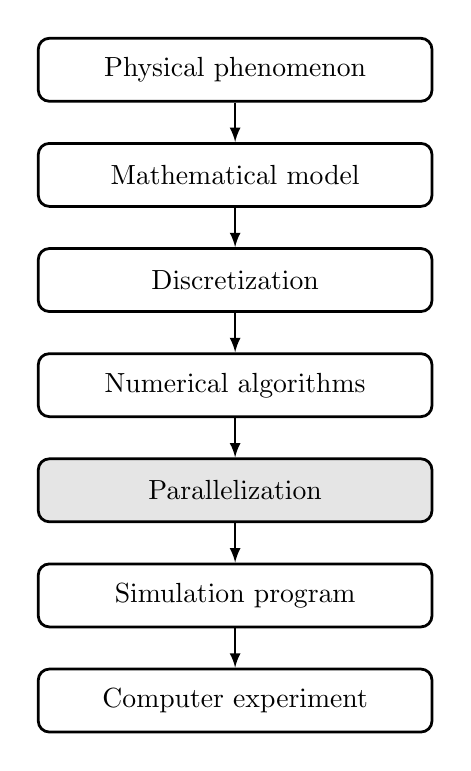
\begin{tikzpicture}[>=latex,thick]
	\matrix (m) [
		matrix of nodes,
		column sep=5mm,
		row sep=5mm,
		nodes={
			draw, % General options for all nodes
			line width=1pt,
			anchor=center,
			text centered,
			rounded corners,
			minimum width=5cm,
			minimum height=8mm,
		},
		txt/.style={text width=1.5cm,anchor=center},
	]
	{
		Physical phenomenon \\
		Mathematical model \\
		Discretization \\
		Numerical algorithms \\
		|[fill=black!10]| Parallelization \\
		Simulation program \\
		Computer experiment \\
	};
	\foreach \i [evaluate={\j=int(\i+1)}] in {1,...,6}{
		\draw[->] (m-\i-1) -- (m-\j-1);
	}

\end{tikzpicture}
}
\caption{Principal steps in computer experiment}
\label{fig:structure}
\end{wrapfigure}

The structure of the document follows the diagram shown in the 
figure~\ref{fig:structure}. In chapter~\ref{ch:intro}, plasma is described as a 
physical phenomenon and we focus on the relevant properties that we want to 
study, from which we derive a mathematical model.  In 
chapter~\ref{ch:plasma-sim} and~\ref{sec:test}. The discretization of the 
mathematical model allows the computer simulation by using numerical algorithms.

%\chapter{Related work}

The simulation of plasma began with the first simulations in the 1950s with the
John Dawson codes for 1D simulation. In 1965 Hockney and Buneman introduced the
direct Poisson solver, which allowed the first useful electrostatic simulations.
In the 1970s, the theory of electrostatic PIC was developed by Langdon, leading
to the first electromagnetic codes.

Finally, from 1980 to the 90s the two main bibles of particle-in-cell codes were
produced  by B. Langdon and C. Birdsall in 1975 \cite{birdsall} and by Hockney
and Eastwood in 1988 \cite{hockney}.

At the Plasma Theory and Simulation Group of the University of California,
Berkeley the XOOPIC \cite{xoopic} family of well known codes were released in
the 1990s.

The are a lot of specific PIC codes which are currently used for the simulation
of various phenomena, mostly centered in fusion reactors: ELMFIRE, GENE, GTC,
ORB5, PAR-T and EUTERPE \cite{euterpe}.



%\part{Theory}%\\ \small \textit{No C code here}}

% What is a plasma: write about the physical phenomenon
%\chapter{Plasma introduction}
\label{ch:plasma-intro}

% Write about how plasma can be simulated with a computer. The methods regarding 
% *only* on numerical methods to simulate plasma, not the specific to HPC ones.

\section{Everyday plasmas}

It may be surprising to find out that when we look at the universe, the most
common state of matter is plasma, which is a ionized gas formed by free
electrons and ions at a region in space--often known as the fourth state of
matter. The sun, our closest star, is a giant
ball of plasma 


Most common forms of plasma only occur in vaccum, as otherwise the air cools the
plasma and returns to a gas.

In our planet, we can see forms of plasma almost every day. A storm day the
lightnings. The spark on some piezoelectric lighters, which is the very same
principle that occurs in gasoline engines.

The Aurora Borealis, of the lightning of a fluorescent tube or the pixels of a
plasma TV.

A precise definition of a plasma is given by Chen~\cite{chen} as \textit{``a
quasineutral gas of charged and neutral particles which exhibits collective
behavior''}. The 


% Begin the simulation of plasma part
\chapter{Plasma simulation}
\label{ch:plasma-sim}

% Write about how plasma can be simulated with a computer. The methods regarding 
% *only* on numerical methods to simulate plasma, not the specific to HPC ones.

\section{The particle-in-cell method}

%TODO: Show the main equation
Solving the Vaslov equation requires a large amount of numerical resources. The 
particle in cell method, approximates the solution by discretization of the 
fields.

The method is divided in four main phases: 

\begin{itemize}
\item Particle motion.
\item Charge accumulation.
\item Solve field equation.
\item Interpolation of fields in particle position.
\end{itemize}


%\section{1D electrostatic simulation}
%The magnetic field is ignored.
%
%\section{2D simulation}
%The magnetic field is not ignored.
%
%\section{Electromagnetism}
%
%\subsection{Background magnetic field}
%
%To introduce the magnetic field, the equations are:
%
%$$ $$

\section{Particle mover}

In order to move the particles, the equations of motion need to be solved:
%
\begin{equation}
m \frac{d\v}{dt} = q (\E + \v \times \B)
\end{equation}
\begin{equation}
\frac{d\v}{dt}=\v
\end{equation}
%
Several methods are available, but we will focus on the Boris integrator.

\subsection{Boris integrator}

Consists of three steps:
%
\begin{enumerate}
\item Add half of the electric impulse
\item Rotate
\item Add the remaining half electric impulse
\end{enumerate}
%
The Boris integrator computes the velocity of a particle in a constant electric 
field $\E$ and a constant magnetic field $\B$. We have the velocity 
$\v_{t-\Delta t/2}$ of the particle at $t-\Delta t/2$ as we use the leapfrog 
integrator.
%
\begin{figure}[h]
\centering
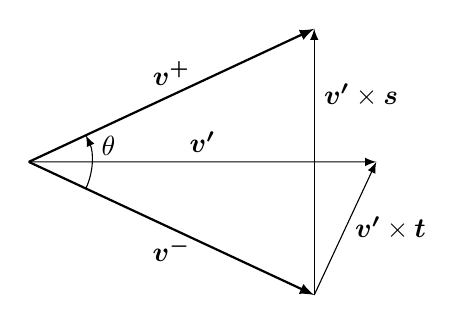
\begin{tikzpicture}[
	scale=2,
	>=latex]

	\def\centerarc[#1](#2)(#3:#4:#5)% Syntax: [draw options] (center) (initial angle:final angle:radius)
		{\draw[#1] ($(#2)+({#5*cos(#3)},{#5*sin(#3)})$) arc (#3:#4:#5); }

	\def\startangle{-25}
	\def\midangle{0}
	\def\endangle{25}
	\def\radius{2.0}
	\pgfmathsetmacro{\vlen}{\radius*tan(\startangle)}%

	\coordinate (O) at (0,0);
	\coordinate (S) at (\startangle:\radius);
	\coordinate (E) at (\endangle:\radius);

%	\centerarc[dashed](O)(\startangle:\endangle:\radius);
	\centerarc[->](O)(\startangle:\endangle:0.2*\radius);

	\draw (O)+(0.4,0.1) node [right] {$\theta$};

	\draw [thick,->] (O) -- (E) node [midway, above] {$\V{v^+}$};
	\draw [thick,->] (O) -- (S) node [midway, below] {$\V{v^-}$};

	\path (S) +(\startangle-90:\vlen) coordinate (V1E);
%	\path (E) +(\endangle-90:\vlen) coordinate (V3E);

%	%\draw [->] (E) -- (V3E);
	\draw [->] (S) -- (V1E) node [midway, right] {$\V{v'} \times \V t$};
%
	\draw [->] (O) -- (V1E) node [midway, above] {$\V{v'}$};
	\draw [->] (S) -- (E) node [near end, right] {$\V{v'} \times \V s$};

%	\draw [fill=white] (O) circle (0.02);

\end{tikzpicture}
\caption{Velocity space rotation from $\v-$ to $\v+$}
\end{figure}
%
\paragraph{Add half electric impulse} We define $\V{v^-}$ as the velocity after 
half a electric impulse:
$$\v^- = \v_{t-\dt/2} + \frac{q \E}{m} \frac{\dt}{2}$$

\paragraph{Rotate for the magnetic field} The rotation is done in two steps, 
first the half rotation is computed, with an angle of $\theta/2$:
$$\v' = \v^- + \v^- \times \V t $$

Then the rotation is completed by symmetry, using the $\V s$ vector
$$ \V s = \frac{2 \V t}{1 + \V t^2} $$
as
$$ \V{v^+} = \V{v^-} + \V{v}' \times \V{s} $$

\section{Charge accumulation}

The charge density $\rho$ is a scalar field

\section{Field equations}

Once we have the charge density $\rho$ we can compute the electric field $\E$ by 
the integration of the field equations
%
\begin{equation}
\E = -\nabla \phi
\end{equation}
\begin{equation}
\nabla \cdot \E = \frac{\rho}{\epsilon_0}
\end{equation}
%
Which can be combined into the Poisson equation
%
\begin{equation}
\label{eq:poisson}
\nabla^2\phi = - \frac{\rho}{\epsilon_0}
\end{equation}
%
Different methods can be used to obtain the electric field, but we will focus on 
matrix and spectral methods.


\chapter{Discrete model}
\label{ch:discrete-model}

\epigraph{... all models are approximations. Essentially, all models are wrong, but some
are useful. However, the approximate nature of the model must always be borne in
mind....}{Empirical Model-Building and Response Surfaces, 1987---George E. P.  
Box}

The mathematical model is discretized in algebraic operations, in order to be 
computable.

\section{Charge assignment}
At each grid point $g$ at $\x$ we accumulate the charge of each particle $p$ in 
$\x_p$ as
%
\begin{equation}%{{{
\rho(\x) = \sum_p q\,W(\x - \x_p) + \rho_0
\label{eq:charge-accumulation}
\end{equation}%}}}
%
The background charge density $\rho_0$ is used to neutralize the total charge 
when is non-zero. The weighting function $W$ determines the shape of the 
particle charge. Different schemes can be used to approximate the charge density 
from the particles. We will focus on bilinear interpolation for it's simplicity 
and low computation requirements. The corresponding weighting function can be 
written as
%
\begin{equation}%{{{
W(\x) =
\begin{cases}
			\displaystyle\left(1 - \frac{|x|}{\Delta x}\right)
				\left(1 - \frac{|y|}{\Delta y}\right) & \text{if}\ -\Delta\x < \x < 
				\Delta \x\\
			0 & \text{otherwise}
\end{cases}
\end{equation}%}}}
%
Notice that a particle $p$ always affects the four enclosing grid points in the 
neighbourhood $\neigh{p}$, but more complex interpolation methods may extend the 
update region even further. It may be noted that the increase in smoothing, at 
computation expense, can gain from the reduced number of particles needed to 
obtain a similar result, avoiding nonphysical effects.
%
\begin{figure}[]%{{{
\centering
\begin{tikzpicture}[
		>=latex,
		effect/.style={dashed,-{Latex[length=3mm, width=1mm]}},
		particle/.style={fill=black,radius=3pt},
	]
	\draw [step=2cm,dotted] (1,1) grid (5,5);
	\coordinate (p) at (2.5,3.2);
	\coordinate (center) at (3,3);
	\coordinate (A) at ($(center)+(-1,1)$);
	\coordinate (B) at ($(center)+(1,1)$);
	\coordinate (C) at ($(center)+(1,-1)$);
	\coordinate (D) at ($(center)+(-1,-1)$);
	\draw[effect] (p) -- (A);
	\draw[effect] (p) -- (B);
	\draw[effect] (p) -- (C);
	\draw[effect] (p) -- (D);
	\node[above left]  at (A) {$A$};
	\node[above right] at (B) {$B$};
	\node[below right] at (C) {$C$};
	\node[below left]  at (D) {$D$};
	\draw[particle] (p) circle;
	\node[left] at (p) {$p$};
\end{tikzpicture}
\hspace{0.5cm}
\begin{tikzpicture}[
		>=latex,
		box/.style={black},
		particle/.style={fill=black,radius=3pt},
		div/.style={dashed},
	]
	\draw [step=2cm,dotted] (1,1) grid (5,5);
	\coordinate (p) at (2.5,3.2);
	\coordinate (center) at (3,3);
	\coordinate (A) at ($(p)+(-1,1)$);
	\coordinate (B) at ($(p)+(1,1)$);
	\coordinate (C) at ($(p)+(1,-1)$);
	\coordinate (D) at ($(p)+(-1,-1)$);
	\draw[box] (A) -- (B) -- (C) -- (D) -- (A);
	\draw[div] ($(A)!(center)!(B)$) -- (center);
	\draw[div] ($(B)!(center)!(C)$) -- (center);
	\draw[div] ($(C)!(center)!(D)$) -- (center);
	\draw[div] ($(D)!(center)!(A)$) -- (center);
	\node at ($(center)!0.5!(A)$) {$a$};
	\node at ($(center)!0.5!(B)$) {$b$};
	\node at ($(center)!0.5!(C)$) {$c$};
	\node at ($(center)!0.5!(D)$) {$d$};
	\draw[particle] (p) circle;
\end{tikzpicture}
\hspace{0.5cm}
\begin{tikzpicture}[
		>=latex,
		box/.style={black},
		particle/.style={fill=black,radius=3pt},
		div/.style={dashed},
	]
	\draw [step=2cm,dotted] (1,1) grid (5,5);
	\coordinate (p) at (2.5,3.2);
	\coordinate (center) at (3,3);
	\coordinate (A) at ($(center)+(-1,1)$);
	\coordinate (B) at ($(center)+(1,1)$);
	\coordinate (C) at ($(center)+(1,-1)$);
	\coordinate (D) at ($(center)+(-1,-1)$);
	\draw[box] (A) -- (B) -- (C) -- (D) -- (A);
	\draw[div] ($(A)!(p)!(B)$) -- (p);
	\draw[div] ($(B)!(p)!(C)$) -- (p);
	\draw[div] ($(C)!(p)!(D)$) -- (p);
	\draw[div] ($(D)!(p)!(A)$) -- (p);
	\node at ($(p)!0.5!(A)$) {$c$};
	\node at ($(p)!0.5!(B)$) {$d$};
	\node at ($(p)!0.5!(C)$) {$a$};
	\node at ($(p)!0.5!(D)$) {$b$};
	\draw[particle] (p) circle;
\end{tikzpicture}
\caption{Interpolation of particle $p$ charge into the four grid points A to D.}
\label{fig:interpolation}
\end{figure}%}}}
%
The particle $p$ has a uniform charge area, centered at the particle position 
$\x_p$, with size $\Delta \x$, as shown in the figure~\ref{fig:interpolation}.  
Each grid point $A,B,C$ and $D$ receives the amount of charge weighed by the 
area $a,b,c$ and $d$. It can be observed that the area is equal to the opposite 
region, when the particle $p$ is used to divide the grid cell.
%
The particle shape can be altered later in the Fourier space, without large 
computation effort, in case the solver already computes the FFT.
%
\section{Field equations}

In order to compute the electric field $\E$, the electric potential $\phi$ is 
generally needed, which can be obtained from the charge density $\rho$.

\subsection{Electric potential}
Several methods are available to solve the Poisson equation 
(Eq.~\ref{eq:poisson}).

\paragraph{Iterative  methods} such as Jacobi, Gauss-Seidel, Successive Over 
Relaxation (SOR), Chebyshev acceleration are some of the most familiar methods 
to solve the Poisson equation.

\paragraph{Matrix methods} The equations from finite differencing the mesh are 
considered a large system of equations. We can find in this methods the Thomas 
Tridiagonal algorithm, Conjugate-Gradient, LU or Incomplete Decomposition.

\paragraph{Spectral methods} Also known as Rapid Elliptic Solvers (RES) are a 
family of methods that use the fast Fourier transform (FFT). Are know for being 
usually faster than the previous ones, with a complexity in $O(N_g \log_2 N_g)$

\vspace{1em}
\noindent
%
We will only focus on the LU for small problems and for testing, and spectral 
methods, more specific on the Multiple Fourier Transform (MTF) method, as it is 
the main method implemented in the simulator, due to its relative simplicity and 
low computational complexity.

\subsection{LU decomposition}
%
% TODO: Check the error bound
For two dimensions, we can approximate the solution using the second order 
centered finite differences (with an error proportional to $\Delta x ^2 \Delta 
y^2$), as
%
\begin{equation}%{{{
\label{eq:discrete-poisson}
\frac{\phi(x-1, y) + \phi(x, y-1) - 4\phi(x,y) + \phi(x+1,y)+\phi(x,y+1)}{\Delta 
x ^2 \Delta y^2} = - \frac{\rho(x,y)}{\epsilon_0}
\end{equation}%}}}
%
which leads to a system of $N_g$ linear equations and can be also written in 
matrix form
%
\begin{equation}
\label{eq:eq-system}
A\phi = -\frac{\Delta x ^2 \Delta y^2\,\rho}{\epsilon_0}
\end{equation}
%
The $N_g \times N_g$ coefficient matrix $A$ has non-zero coefficients only at 
$a_{ii} = 4$ and $a_{ij} = -1$ with $j \in \{i+1, i-1, i+N_x, i-N_x\} \mod N_x$, 
for all $0 \le i \le Ng$.
%
However, the matrix $A$ is singular, so the system of equations has infinite 
solutions. Boundary conditions can be added to get a unique solution. The extra 
equation $\phi(0,0) = 0$ leads to a system with only one solution, but with one 
extra equation. In order to keep the matrix $A$ square, the following steps may 
be taken:

\begin{enumerate}
\item Subtract  the extra equation $\phi(0,0) = 0$ to the first row of $A$, with 
the only change in the coefficient to $a_{11} = 3$.

\item Add all first $N_g$ equations: Each equation has one coefficient of $4$ 
and four of $-1$ except the first equation. Also we assume the total charge 
density is zero, obtaining $\phi(0,0) = 0$.

\item Subtract it from the last equation, which leads to a zero coefficient that 
can be removed.
\end{enumerate}
%
The only change that remains is at the coefficient $a_{11} = 3$. Now the matrix 
$A$ is squared and non-singular and has only one solution and can now be solved 
with the $LU$ method.

The $LU$ decomposition, with a complexity in $O(2/3N_g^3)$, can be used to form 
two systems of equations that can be solved faster. If we rewrite the system of 
equations~\ref{eq:eq-system} as the usual form $Ax=b$ with
\begin{equation}
x = \phi,\quad b = -\frac{\Delta x ^2 \Delta y^2\,\rho}{\epsilon_0}
\end{equation}
%
Then we can use the decomposition $A=LU$ to form two systems of equations
%
\begin{equation}
\label{eq:LU-systems}
Ux=y, \quad Ly=b
\end{equation}
%
which can be solved in complexity $O(2N_g^2)$.


\subsection{Multiple Fourier Transform (MFT)}

The general second-order PDE with constant coefficients and periodic boundary 
conditions
%
\begin{equation}%{{{
\label{eq:gen-fd}
a \frac{\partial^2 \phi}{\partial x^2}+b\frac{\partial \phi}{\partial x}+c\phi +
d \frac{\partial^2 \phi}{\partial y^2}+e\frac{\partial \phi}{\partial y}+f\phi = 
g(x,y)
\end{equation}%}}}
%
can be solved by using the FFT. If we expand $\phi$ and $g$ in a finite double 
Fourier series, we obtain
%
\begin{equation}%{{{
\phi(x,y) = \sum_{k,l} \hat \phi(k, l) \exp\left({\frac{2\pi i (xk + 
yl)}{n}}\right)
\end{equation}%}}}
%
and
%
\begin{equation}%{{{
g(x,y) = \sum_{k,l} \hat g(k, l) \exp\left({\frac{2\pi i (xk + yl)}{n}}\right)
\end{equation}%}}}
%
which now can be substituted in the Eq.~\ref{eq:gen-fd}, to obtain
%
\begin{equation}%{{{
\hat \phi(k,l) = \hat G(k,l) \, \hat g(k,l),\quad 0<k<N_x,\,0<l<N_y
\end{equation}%}}}
%
with for a unit mesh
%
\begin{equation}%{{{
\begin{split}
\hat G(k,l) = \Bigg[
& 2a \left( \cos \frac{2\pi k}{n} - 1 \right) +
ib \sin \frac{2\pi k}{n} + c \,+ \\
& 2d \left( \cos \frac{2\pi l}{n} - 1 \right) +
ie \sin \frac{2\pi l}{n} + f
\Bigg]^{-1}
\end{split}
\end{equation}%}}}
%
To solve the Poisson equation, discretized as Eq.~\ref{eq:discrete-poisson}, we 
have $a=d=1$ and $b=c=e=f=0$ so we can simplify $\hat G(k,l)$ as
%
\begin{equation}%{{{
\hat G(k,l) = \frac{1}{2}\left[
\cos \frac{2\pi k}{n} +
\cos \frac{2\pi l}{n} -
2 \right]^{-1}
\end{equation}%}}}
%
Let $g = -{\Delta x ^2 \Delta y^2\,\rho}/{\epsilon_0}$, then the steps to 
compute the electric potential can be summarized as follows:
%
\begin{center}%{{{
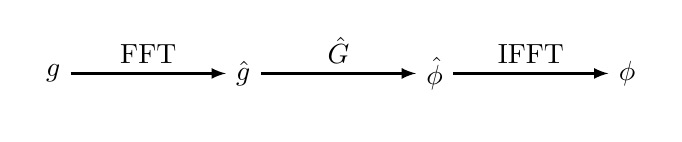
\begin{tikzpicture}[>=latex,thick]
	\matrix (m) [
		matrix of nodes,
		column sep=20mm,
		nodes={
			%line width=1pt,
			anchor=center,
			text centered,
			%minimum width=1cm,
			minimum height=8mm,
		},
%		txt/.style={text width=1.5cm,anchor=center},
	]
	{
		$g$ & $\hat g$ & $\hat \phi$ & $\phi$ \\%& $\E$\\
	};
	\foreach \i [evaluate={\j=int(\i+1)}] in {1,...,3}{
		\draw[->] (m-1-\i) -- (m-1-\j);
	}
	\draw[draw=none] (m-1-1) -- (m-1-2) node[midway,above] {FFT};
	\draw[draw=none] (m-1-2) -- (m-1-3) node[midway,above] {$\hat G$};
	\draw[draw=none] (m-1-3) -- (m-1-4) node[midway,above] {IFFT};
%	\draw[draw=none] (m-1-4) -- (m-1-5) node[midway,above]
%	{Eq.~\ref{eq:phi-to-E}};
\end{tikzpicture}
\end{center}%}}}
%
\begin{enumerate}
\item Compute the complex FFT $\hat g$ of $g$
\item Multiply each element of $\hat g$ by the corresponding complex coefficient 
$\hat G$, to obtain $\hat \phi$
\item Compute the inverse FFT of $\hat \phi$ to get $\phi$
\end{enumerate}
%
The complexity in the worst case is in $O(N_g \log_2 N_g)$ with the number of 
total points in the grid $N_g$.

\subsection{Electric field}
The electric field $\E$ can then be obtained by centered first order finite 
differences in each dimension
%
\begin{equation}%{{{
\begin{split}
\label{eq:phi-to-E}
\E_x(x,y) &= \frac{\phi(x-1,y) - \phi(x+1,y)}{2\,\Delta x} \\
\E_y(x,y) &= \frac{\phi(x,y-1) - \phi(x,y+1)}{2\,\Delta y}
\end{split}
\end{equation}%}}}
%

\section{Force interpolation}

The force acting on a particle $p$ can be decomposed in two main parts, the 
electric and magnetic force $\F=\F_E + \F_B$.

The electric force $\F_E$ is computed similarly as the charge deposition, but in 
the reverse order. The force $\F_E$ is interpolated from the electric field $\E$ 
of the neighbour grid points $\neigh{p}$, using the same interpolation function 
$W$.
\begin{equation}%{{{
\begin{split}
\F_E &= q \sum_{g \in \neigh{p}} W(\x_p - \x_g)\ \E(\x_g) \\
\end{split}
\end{equation}%}}}
Notice that a particle $p$ only needs the values of the electric field in the 
neighbourhood $\neigh{p}$.

The magnetic force $\F_B$ is constant in the simulator, as we only consider a 
fixed background magnetic field $\B_0$. For a particle $p$ with velocity $\v$  
can be written as
%
\begin{equation}%{{{
\F_B = q (\v \times \B_0)
\end{equation}%}}}


\section{Equations of motion}

In order to move the particles, the equations of motion need to be solved:
%
\begin{equation}
\frac{d\x}{dt}=\v
\end{equation}
\begin{equation}
m \frac{d\v}{dt} = \F
\end{equation}
%
The \textit{leap-frog} method is a common integration scheme with second-order 
accuracy and an error proportional to $\Delta t^2$. The name describes de 
behavior of the position and velocity, which are updated at interleaved time 
steps, similarly to the trajectory of a frog. The method is time reversible with 
an stability far superior of other higher-order integration methods, such as 
fourth order Runge-Kutta. A more in depth stability analysis can be found in 
Chapter 4 of Hockney and Eastwood book~\cite{hockney}.  The discretized 
equations can be written as
%
\begin{equation}
\frac{\x^{n+1} - \x^{n}}{\Delta \x} = \v^{n + 1/2}
\end{equation}
%
\begin{equation}
m\frac{\v^{n+1/2} - \v^{n-1/2}}{\Delta \x} = \F(x^n)
\end{equation}
%
Several methods are available, but we will focus on the Boris integrator.

\subsection{Boris integrator}

Consists of three steps:
%
\begin{enumerate}
\item Add half of the electric impulse
\item Rotate
\item Add the remaining half electric impulse
\end{enumerate}
%
The Boris integrator computes the velocity of a particle in a constant electric 
field $\E$ and a constant magnetic field $\B$. We have the velocity 
$\v_{t-\Delta t/2}$ of the particle at $t-\Delta t/2$ as we use the leapfrog 
integrator.
%
\begin{figure}[h]
\centering
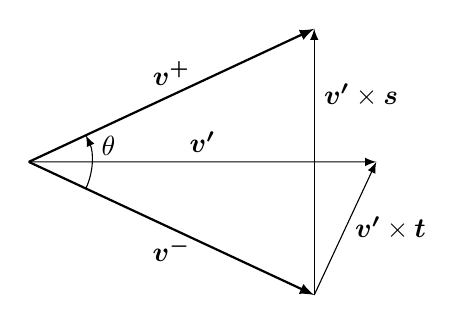
\begin{tikzpicture}[
	scale=2,
	>=latex]

	\def\centerarc[#1](#2)(#3:#4:#5)% Syntax: [draw options] (center) (initial angle:final angle:radius)
		{\draw[#1] ($(#2)+({#5*cos(#3)},{#5*sin(#3)})$) arc (#3:#4:#5); }

	\def\startangle{-25}
	\def\midangle{0}
	\def\endangle{25}
	\def\radius{2.0}
	\pgfmathsetmacro{\vlen}{\radius*tan(\startangle)}%

	\coordinate (O) at (0,0);
	\coordinate (S) at (\startangle:\radius);
	\coordinate (E) at (\endangle:\radius);

%	\centerarc[dashed](O)(\startangle:\endangle:\radius);
	\centerarc[->](O)(\startangle:\endangle:0.2*\radius);

	\draw (O)+(0.4,0.1) node [right] {$\theta$};

	\draw [thick,->] (O) -- (E) node [midway, above] {$\V{v^+}$};
	\draw [thick,->] (O) -- (S) node [midway, below] {$\V{v^-}$};

	\path (S) +(\startangle-90:\vlen) coordinate (V1E);
%	\path (E) +(\endangle-90:\vlen) coordinate (V3E);

%	%\draw [->] (E) -- (V3E);
	\draw [->] (S) -- (V1E) node [midway, right] {$\V{v'} \times \V t$};
%
	\draw [->] (O) -- (V1E) node [midway, above] {$\V{v'}$};
	\draw [->] (S) -- (E) node [near end, right] {$\V{v'} \times \V s$};

%	\draw [fill=white] (O) circle (0.02);

\end{tikzpicture}
\caption{Velocity space rotation from $\v-$ to $\v+$}
\end{figure}
%
\paragraph{Add half electric impulse} We define $\V{v^-}$ as the velocity after 
half a electric impulse:
$$\v^- = \v_{t-\dt/2} + \frac{q \E}{m} \frac{\dt}{2}$$

\paragraph{Rotate for the magnetic field} The rotation is done in two steps, 
first the half rotation is computed, with an angle of $\theta/2$:
$$\v' = \v^- + \v^- \times \V t $$

Then the rotation is completed by symmetry, using the $\V s$ vector
$$ \V s = \frac{2 \V t}{1 + \V t^2} $$
as
$$ \V{v^+} = \V{v^-} + \V{v}' \times \V{s} $$


%\part{Computation}%\\ \small \textit{No more physics now}}

\chapter{Sequential simulator}
\label{ch:sequential}

\epigraph{The purpose of computation is insight, not numbers.}{Numerical Methods 
for Scientists and Engineers, 1962---Richard Hamming}

In order to begin the implementation of the simulator, an initial version was
considered with the minimum complexity, to verify the correctness of the model.
A graphic subsystem was build with MathGL and OpenGL to produce realtime plots
of different elements of the simulation. Of special interest are the particle
motion, the electric potential and the electric field.

The language of choice was C for the low overhead, the lack of automatic memory
management, the support of different libraries planned in future versions and
the low level design, which allowed us to define most of the data structures
close to the byte level.

\section{Design}

The simulator initially only supported one group of particles of the same charge
and mass, denominated specie. Each particle was implemented as a structure with
a given index $i$, a position vector $\x$, velocity $\v$ and other extra fields
such as the interpolated electric field at the particle position $\E$.
%
Only one dimension was implemented for the first tests, but soon extended to two 
dimensions.  The fields were allocated in contiguous arrays, with the $x$ 
dimension aligned with the cache line, also called row-major storage.

The configuration of the simulation is specified in plain configuration files, 
with the syntax defined by the \texttt{libconfig} library. It is important to 
allow the user to specify comments in the configuration files, as well as 
scientific notation in different values. Additionally, the specification of 
multiple species benefits from the sub-configuration block feature, which leads 
to a more intuitive representation.

The solver used was initially the $LU$ decomposition, used from the $GSL$
numeric library~\cite{gsl}, as the only focus was to obtain valid results, ignoring the
performance. All implementations are tested beforehand with some test cases
designed in \texttt{octave}.

\subsection{Debug mode}

In order to get insight into all the details of the simulation, a mechanism of 
visualization can be very useful: the different fields can be plotted in 
real-time for one and two dimensions, while the particles move around. The 
simulator includes a visualization mode, in which the state of the simulation is 
plotted at a specific period of iterations (by default each iteration is shown).  
In this mode (which we will refer to as debug mode) the simulation is slowed 
down, with a top speed of 60 iterations per second, to follow the visualization 
in the screen.


%
\begin{figure}[h]
	\centering
	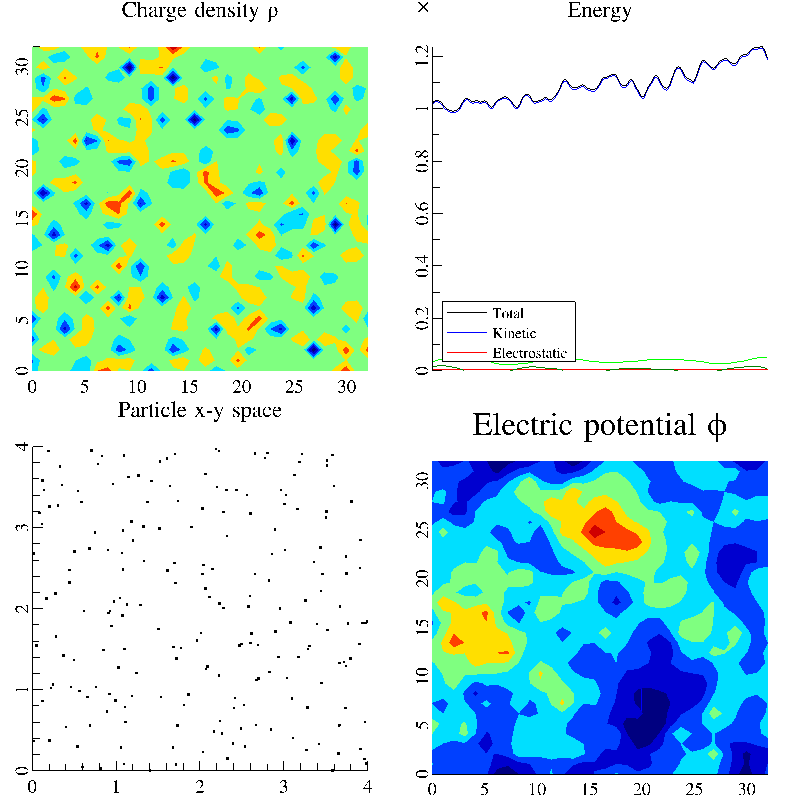
\includegraphics[width=0.95\linewidth]{sim.png}
	\label{fig:debug-mode}
	\caption{Example run in 2D of the simulator in debug mode.}
\end{figure}

With this mode activated, the user can observe and quickly check the overall 
behavior of the simulation, as is designed to minimize the delay between writing 
the configuration of the simulation and the execution. Once the simulator is 
running, the user can see several graphs being updated as shown in the 
figure~\ref{fig:debug-mode}.

The energy measurements are always shown, including potential, kinetic and total 
energy---the total energy must be conserved at all times. In the case of 
one-dimensional simulations, the particles are plotted in the $x$-$v$ phase 
space, with the fields aligned vertically. However, in two dimensions the 
particles are plotted by default in the $x$-$y$ plane which corresponds to the 
physical position in space. The fields now cannot be plotted together, an only 
the electric potential is shown.

Once the simulation is properly tested in the debug mode, there is less chance 
that a misconfigured setting ruins a large simulation. This mode has also being 
very helpful when developing the simulator, as several test required to see the 
immediate result of a new feature, or to change a value in the configuration.

\section{Validation}

A set of different tests were designed to determine the correctness of the
simulation.

\subsection{Two particle test}

A simple one-dimensional test consists of two electrons placed at some distance 
different of $L/2$ with no initial speed. The analytical solution is known and 
the motion should follow a harmonic oscillation trajectory. The energy 
conservation can be observed in the figure~\ref{fig:1d-2particles-energy}, where 
the total energy only varies due to the interpolation noise as the time $t$ 
grows in the $x$ axis.
%
\begin{figure}[h]
	\centering
	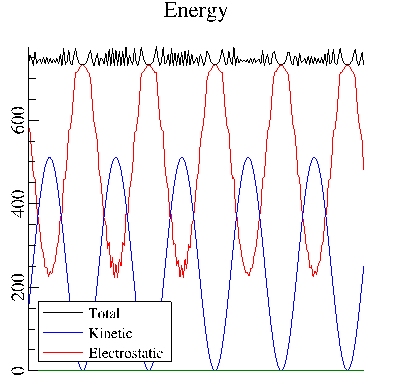
\includegraphics[width=0.4\linewidth]{1d-2particles-energy.png}
	\caption{Energy conservation in two particle test as shown in the simulator 
	(notice the lack of anti-aliasing).}
	\label{fig:1d-2particles-energy}
\end{figure}

\subsection{Two stream instability}

%
\begin{figure}[ht]
	\centering
	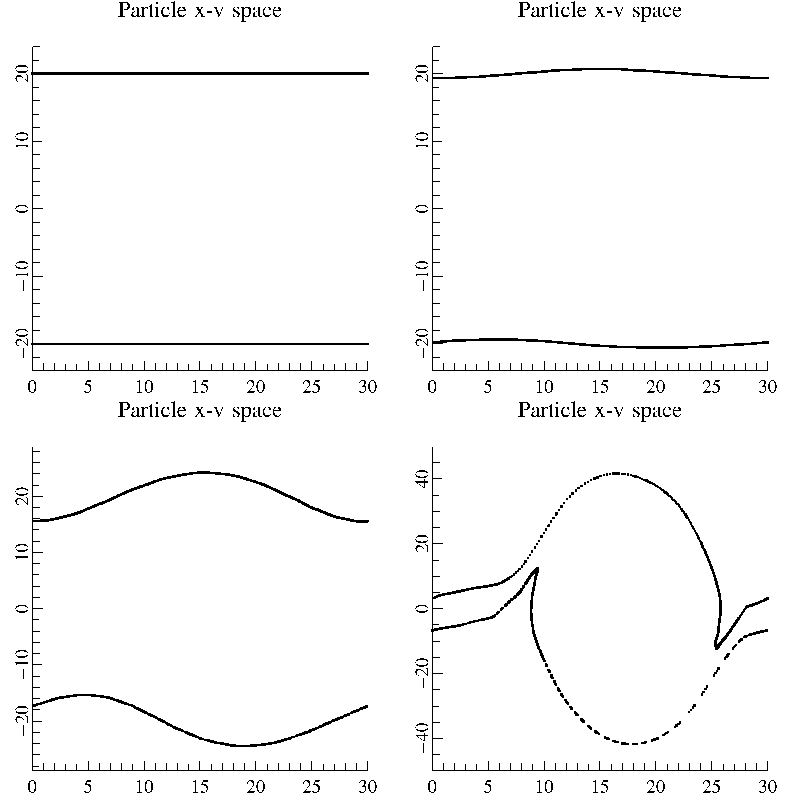
\includegraphics[width=0.8\linewidth]{1d/2stream/out.png}
	\caption{Phase space position--velocity of the two stream instability, shown 
	at iterations: 0, 200, 400 and 600 (left to right, top to bottom)}
	\label{fig:1d-2stream}
\end{figure}

Another example in one dimension is the two stream instability, which consists 
of two streams of particles with opposite velocity. With 500 particles in each 
stream, a very characteristic set of vortices are created in the 
position-velocity phase space, which can be shown in the 
figure~\ref{fig:1d-2stream}.

\subsection{Cyclotron frequency}

In a simulation with two dimensions and a fixed background magnetic field 
$\B_0$, a charged particle with some initial velocity should describe a circular 
orbit. The radius $r_g$ known as the Larmor or gyroradius, can be computed 
analytically as
\begin{equation}
r_g = \frac{m v}{|q| B}
\end{equation}

\chapter{Parallelization techniques}
\label{ch:techniques}

\section{Message Passing Interface}

From the need of standarize communications in a distributed computing
environment, the first draft was proposed in 1992 at the Workshop on Standards
for Message Passing in a Distributed Memory Environment, and has now become one
of the most used communication protocol in HPC. The Message Passing Interface
(MPI) provides a simple to use set of routines to allow processes distributed
among different nodes to comunicate efficiently.

\subsection{Concepts}


\paragraph{Communicator} A communicator refers to a group of processes, in which
each has assigned a unique identifier called the \textit{rank}.

\paragraph{Point-to-point communication} In order for a process to exchange
information with another process, the MPI standard defines what are called
point-to-point communication routines. The most common examples are
\texttt{MPI\_Send} to send data, and \texttt{MPI\_Recv} for the reception.
Both routines need the process rank of the process to stablish the connection.
Additionally a tag is used to label each message, which can be specified in the
reception to filter other messages.

\paragraph{Blocking communication} The standard defines various types of
communication methods for sending and receiving data. The so called blocking
routines are designed such that the call does not return until the communication
has been done. In the \texttt{MPI\_Send} case, the call returns when the sending
data can be safely modified, as has been sent or buffered. In the case of
\texttt{MPI\_Recv} the routine only returns when the data has been received.

\paragraph{Non-blocking communication} Similarly as with the blocking
communication, the routines \texttt{MPI\_Isend} and \texttt{MPI\_Irecv} don't
wait until the message is sent or received to return. They return inmediately,
and the communication status can be checked with \texttt{MPI\_Test} or the
process can wait until the communication request has finished with
\texttt{MPI\_Wait}.

\subsection{Implementations}


\section{OmpSs-2}

OmpSs-2 is the next generation of the OmpSs programming model, composed of a set
of directives and library routines. Mixes from OpenMP the annotation of source
code to parallelize some sections with the StarSs execution model, based on a
data-flow execution model.

\subsection{Concepts}

\paragraph{Task} In OmpSs-2 a task is a section of code that can be executed
independently by the runtime schedule. A task may have associated dependencies
which lets the scheduler determine in wich order is allowed to execute the
tasks. The notation used to describe a task is by the utilization of the
\texttt{\#pragma} directive, for example:
%
\begin{lstlisting}
#pragma oss task inout(a[0:N-1]) in(b[0:N-1])
for(i=0; i < N; i++)
	a[i] += b[i];
\end{lstlisting}
%

\paragraph{Parallel execution} Unless there is a unmet dependency, all tasks 
ready to run are executed in parallel, up to the number of CPU cores available 
to the runtime.

\paragraph{Task syncronization} It may be possible that at some point in the
execution all pending task are required to finish in order to continue. The
directive \texttt{taskwait} allows the programmer to specify that the runtime
must wait for completion of all previous created tasks.

%\chapter{Simulator design}

[This chapter will be merged with the next one, is only here to keep the
numbering of the chapters, while I'm working on the comments]

\chapter{The simulator}
\label{ch:parallel-simulator}

\section{Decomposition}

To parallelize the simulation, the process must be decomposed in parts that can 
be executed in parallel and several decompositions are known.
%
One of the most common technique found in particle-in-cell codes, is the 
\textit{domain decomposition}---the physical space is divided into sections of 
similar size and the fields are assigned to different computing units. The main 
drawback of this technique is the risk of unbalanced load, as some regions of 
space may contain a large amount or even all the particles.

Another approach called \textit{particle decomposition} consists in the division 
of the particles into groups, where each processor maintains a copy of the 
fields of the whole space.  The problem of this method is the limitation of 
scalability, as the number of grid points used in the fields is limited by the 
memory of one computing element.

Additionally, the Fourier transform needed by the MFT solver is implemented 
using the FFTW library and the parallelization design provided by the library 
introduces a constraint in the distribution of the fields: they need to be 
broken into slices in the Y dimension, resulting in contiguous blocks of 
elements in X. Consequently, the domain decomposition is the chosen technique 
for the simulator.

\begin{figure}[ht]%{{{
\centering
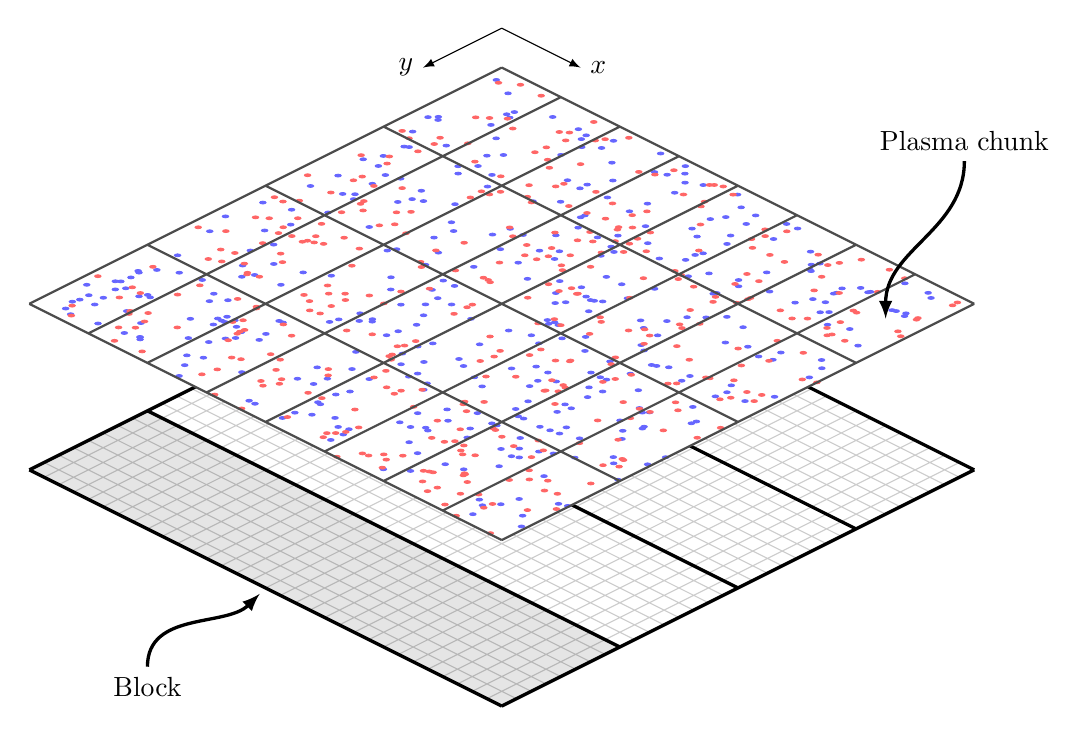
\begin{tikzpicture}
\begin{scope}[
		x=1cm,
		y=1cm,
		yshift=0,
		every node/.append style={
			yslant=0.5,xslant=-1},
		yslant=0.5,
		xslant=-1
	]
	% opacity to prevent graphical interference
	\draw[step=1.5/8, black!20!white, thin] (0,0) grid (6,6); %defining grids
	%\draw[step=1.5, black] (0,0) grid (6,6);
	\draw[xstep=1.5, ystep=6, black, very thick] (0,0) grid (6,6);
	%\draw[dashed, xstep=6, ystep=1.5, black] (0,0) grid (6,6);
	\fill[fill=black,fill opacity=0.1] (0,0) rectangle (1.5,6);
	\coordinate (a0) at (4.5, 0);
	\coordinate (a1) at (6, 0);
	\coordinate (a2) at (4.5, 1.5);
	\coordinate (a3) at (6, 1.5);

	\coordinate (b) at (0,3);

\end{scope}
\begin{scope}[
		x=1cm,
		y=1cm,
		yshift=60,
		every node/.append style={
			yslant=0.5,xslant=-1},
		yslant=0.5,
		xslant=-1
	]
	\coordinate (b0) at (4.5, 0);
	\coordinate (b1) at (6, 0);
	\coordinate (b2) at (4.5, 1.5);
	\coordinate (b3) at (6, 1.5);
	\coordinate (c) at (4.5+0.75, 0.75/2);
	%Idem as above, for the n-th grid:
%	\draw[dotted] (a0) -- (b0);
%	\draw[dotted] (a1) -- (b1);
%	\draw[dotted] (a2) -- (b2);
%	\draw[dotted] (a3) -- (b3);
%
%	\draw[dashed] (a2) -- (a3);

	\fill[fill=white,fill opacity=1.0] (0,0) rectangle (6,6);
	\begin{axis}[width=7.5cm,height=7.5cm,
						axis lines=none,
						%hide axis,
						xmin=-1, xmax=1,
						ymin=-1, ymax=1,
						inner frame sep=0,
				]
	\addplot [blue!60!white, only marks,
		mark=*, samples=400, mark size=0.75] (rand, rand);
	\addplot [red!60!white, only marks,
		mark=*, samples=400, mark size=0.75] (rand, rand);
	\end{axis}
	%\draw[step=1.5, black, thick] (0,0) grid (6,6);
	\draw[xstep=1.5, ystep=1.5/2, black!70!white, thick] (0,0) grid (6,6);
	%\draw[dashed,xstep=6, ystep=1.5, black, thick] (0,0) grid (6,6);


	\coordinate (O) at (6.5, 6.5);
\end{scope}

\draw[-latex,very thick] (c)+(1,2) node[above]{Plasma chunk}
				to[out=-90,in=90] (c);
\draw[-latex,very thick,shorten >=3pt] (b)+(-1.5,-1) node[below]{Block}
				to[out=90,in=180+45] (b);

\begin{scope}[
		y={(-1cm,0.5cm)},x={(1cm,0.5cm)}, z={(0cm,1cm)},
	]
%	\coordinate (O) at (-3, 3.5, 0);
%	\draw[-latex] (O) -- +(1, 0,  0) node [right] {$x$};
%	\draw[-latex] (O) -- +(0, -1, 0) node [right] {$y$};
%	\coordinate (O) at (-0.75, -0.75, 0);
	\draw[-latex] (O) -- +(-1, 0,  0) node [left] {$y$};
	\draw[-latex] (O) -- +(0, -1, 0) node [right] {$x$};
\end{scope}
\end{tikzpicture}
\caption{Domain decomposition: The plasma is divided into chunks in both 
directions and the fields into blocks in the Y dimension only}
\label{fig:domain-decomposition}
\end{figure}%}}}

Firstly, the space domain is distributed in blocks by splitting the physical 
space in the Y dimension, as shown in the figure~\ref{fig:domain-decomposition}, 
and each block is assigned to an MPI process. As the simulation evolves, 
communications are needed to exchange information between processes. The 
particles enclosed within a block also are assigned to the same process in order 
to speed up the interpolation process. Furthermore, a second level of 
decomposition splits the particles of a process into plasma chunks, which can be 
processed in parallel. In this case communications within the chunks of a 
process are not needed as we can use shared memory to exchange information.  
Notice that the number of chunks can vary to fit the number of CPUs.

We will refer to a block to denote the region of space assigned to a process and 
the grid points contained in that region. On the other hand a chunk has also a 
region of space assigned of a block, but always is associated with a group of 
particles.

\section{Data layout}

Each block contains the three fields needed for the simulation: the charge 
density $\rho$, the electric potential $\phi$ and the electric field $\E$, which 
can be decomposed in the two components $E_x$ and $E_y$. As a consequence, a 
total of four matrices are needed to store the three fields.

\begin{figure}[h]%{{{
\centering
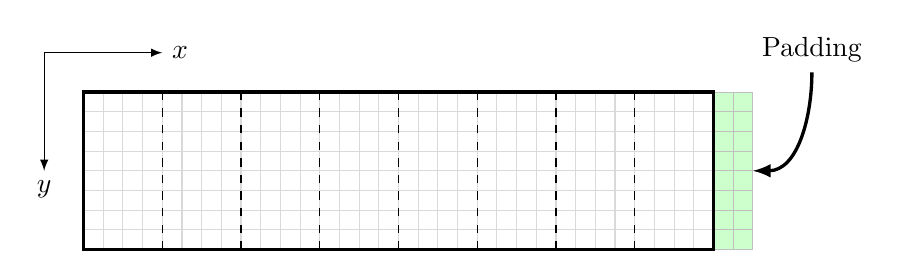
\begin{tikzpicture}[x=0.5cm,y=0.5cm]

\fill[green!20] (16,0) rectangle (17,4);
\draw[gray!30!white,step=0.5] (0,0) grid (16,4);
\draw[gray!50!white,step=0.5] (16,0) grid (17,4);
\draw[dashed,xstep=16/8,ystep=4] (0,0) grid (16,4);
\draw[very thick] (0,0) rectangle (16,4);

\coordinate (pad) at (17, 2);
\draw[-latex,very thick] (pad)+(1.5,+2.5) node[above] {Padding}
				to[out=-90,in=0] (pad);

\coordinate (O) at (-1, 5, 0);
\draw[-latex] (O) -- +(3, 0,  0) node [right] {$x$};
\draw[-latex] (O) -- +(0,  -3, 0) node [below] {$y$};
\end{tikzpicture}
\caption{A block divided in eight regions, each corresponding to a plasma chunk.  
Extra padding is added at the right for internal use in the FFTW library.}
\label{fig:block}
\end{figure}%}}}

A simplified representation of a block can be observed in the 
figure~\ref{fig:block}, where the X dimension of each field is contiguous in 
memory.  Notice the padding region in green, which is needed for the FFTW 
library to store intermediate values. The use of ghost elements is needed for 
communications and will be detailed in the chapter~\ref{ch:comm}. If we look at 
each cell $(x,y)$ in the block we find the four components $\rho(x,y)$, 
$\phi(x,y)$, $E_x(x,y)$ and $E_y(x,y)$.

\section{Simulation flow}

Before the main loop of the simulation begins, two previous iterations are 
required to prepare the simulation. The iteration counter is initially set to 
$-2$ to account for the extra steps.

\subsection{Allocation step}

After the creation of all MPI processes, the different structures to hold the 
data are allocated. Each process is assigned a block, with the corresponding 
fields and particles.

The fields are zeroed to begin the computation and the particles must be 
initialized following the user configuration. Each particle has an index which 
is used to let the user customize the particle attributes in case is required.  
Some initialization functions are provided, which place the particles following 
a random distribution or a specified pattern.

As the particles in a chunk are initialized, their position can set to any point 
in the physical space of the simulation, as no constraints are imposed for the 
initial placement. As a consequence, they need to be translated to the correct 
chunk before the simulation begins. We will refer to the initial movement of 
particles around the chunks as global communication, and is expected to last 
more than the typical communications once the simulation is running, as only 
local communications will be needed between neighbour chunks.

At soon as each particle is properly placed in the correct chunk, an initial 
computation of the charge density is done and the iteration counter is 
incremented.

\subsection{Rewind step}

The main loop begins with an special iteration that will only change the speed 
of the particles. The speed must be computed at half a time-step backwards in 
time, in order to use the leap-frog integrator as described in the 
section~\ref{sec:motion}. Once the iteration finishes, the main loop of can 
begin its normal execution with the iteration counter set to 0.

\subsection{Main loop}

The loop of the simulation performs four main steps:

\begin{itemize}
\item Accumulate charge density $\rho$ from the position of the particles.
\item Solve the field equation to get the electric field $\E$.
\item Interpolate the electric field $\E$ at particle positions.
\item Move the particles based on the computed force.
\end{itemize}

\section{Loop parallelization}

The four main steps of the simulation loop are parallelized following a common 
scheme: the block is partitioned in the same regions as the plasma chunks, which 
are processed in parallel.

\subsection{Charge accumulation}

%\begin{figure}[ht]%{{{
\begin{wrapfigure}{O}[2.7cm]{0.15\textwidth}
\centering
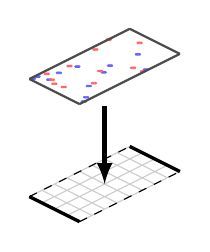
\begin{tikzpicture}[scale=0.85]
\begin{scope}[
		x=1cm,
		y=1cm,
		yshift=0,
		every node/.append style={
			yslant=0.5,xslant=-1},
		yslant=0.5,
		xslant=-1
	]
	\def\dx{0.0};
	% opacity to prevent graphical interference
	\draw[step=1.5/8, black!20!white, thin] (0,0-\dx) grid (6/4,6/8+\dx);
	%defining grids
	%\draw[step=1.5, black] (0,0) grid (6,6);
	\draw[xstep=1.5, ystep=0, black, very thick] (0,0-\dx) grid
		(6/4,6/8+\dx);
	\draw[dashed, xstep=6, ystep=1.5/2, black] (0,0) grid (6/4,6/8);

	\coordinate (b) at (1.5/2, 0.75/2);

\end{scope}
\begin{scope}[
		x=1cm,
		y=1cm,
		yshift=50,
		every node/.append style={
			yslant=0.5,xslant=-1},
		yslant=0.5,
		xslant=-1
	]
	\coordinate (c) at (1.5/2, 0.75/2);

	%\fill[fill=white,fill opacity=1.0] (0,0) rectangle (6,6);
	\begin{axis}[width=3cm,height=2.35cm,
						axis lines=none,
						%hide axis,
						xmin=-1, xmax=1,
						ymin=-1, ymax=1,
						inner frame sep=0,
				]
	\addplot [blue!60!white, only marks,
		mark=*, samples=12, mark size=0.75] (rand, rand);
	\addplot [red!60!white, only marks,
		mark=*, samples=12, mark size=0.75] (rand, rand);
	\end{axis}
	%\draw[step=1.5, black, thick] (0,0) grid (6,6);
	\draw[xstep=1.5, ystep=1.5/2, black!70!white, thick] (0,0) grid (6/4,6/8);
	%\draw[dashed,xstep=6, ystep=1.5, black, thick] (0,0) grid (6,6);


	\coordinate (O) at (1.5+0.5, 0.75+0.5);
\end{scope}

%\draw[-latex,very thick] (c)+(1,2) node[above]{Plasma chunk}
%				to[out=-90,in=90] (c);
%\draw[-latex,very thick,shorten >=3pt] (b)+(-1.5,-1) node[below]{Block}
%				to[out=90,in=180+45] (b);
\draw[-latex,ultra thick,shorten <=0.5cm]
	(c) to[out=-90,in=90] (b);
%	(c) to[out=-90,in=90]  node[midway,right]{Interpolation} (b);

\begin{scope}[
		y={(-1cm,0.5cm)},x={(1cm,0.5cm)}, z={(0cm,1cm)},
	]
%	\coordinate (O) at (-3, 3.5, 0);
%	\draw[-latex] (O) -- +(1, 0,  0) node [right] {$x$};
%	\draw[-latex] (O) -- +(0, -1, 0) node [right] {$y$};
%	\coordinate (O) at (-0.75, -0.75, 0);
%	\draw[-latex] (O) -- +(-1, 0,  0) node [left] {$y$};
%	\draw[-latex] (O) -- +(0, -1, 0) node [right] {$x$};
\end{scope}
\end{tikzpicture}
%\caption{Interpolation of the electric field $\E$ to the particles in a chunk.}
%\label{fig:interpolation-E}
\end{wrapfigure}
%\end{figure}%}}}
%
The interpolation process described in the equation~\ref{eq:charge-accumulation} 
is executed in parallel for all the particles of each chunk. The charge density 
field is being updated in parallel, which involves the four surrounding grid 
points of a particle, and it may happen that at the frontier of two chunks a 
concurrent access to the same element occurs.

To avoid a race condition with the next chunk, a dependency is added with the 
directive \texttt{commutative}, which allows the execution of the tasks in any 
order, but guarantees that a chunk can only be acessed by one task at a time. A 
detailed discussion on the directive can be found in the 
section~\ref{sec:exchange-x} with other alternatives to avoid a chain of 
dependencies in the case \texttt{inout} was used.

\begin{figure}[h]
\begin{lstlisting}[caption={Task to update $\rho$ field using the 
\texttt{commutative} directive}, captionpos=b]
for (i=0; i<plasma->nchunks; i++)
{
	c0 = &plasma->chunks[i];
	c1 = &plasma->chunks[(i + 1) % plasma->nchunks];
	#pragma oss task commutative(*c0, *c1) label(rho_update_0)
	rho_update(sim, i);
}
\end{lstlisting}
\end{figure}
% XXX Notice that we cannot have commutative in the next step or in the previous
% otherwise we can get ot of order execution in a chunk.

\subsection{Solve the fields}

Once the charge density is accumulated for each chunk, the electric potential 
can be computed by solving the Poisson equation (Eq.~\ref{eq:poisson}).  Using 
the MFT solver requires the computation of the Fourier transform of the charge 
density field, which has been purposely distributed among the Y dimension into 
blocks: The computation of the FFT can then be distributed into each process.

To parallelize the execution in each process, two mechanism are available in the 
FFTW library: pthreads and OpenMP. The multithreading design is based on the 
model of the \textit{parallel for}, where the total number of iterations are 
divided into parts that can be executed in parallel.
%
\begin{figure}[ht]%{{{
\begin{lstlisting}[
	%float,
	label={lst:openmp-for},
	caption={Parallel for with OpenMP used in the FFTW library.}]
#pragma omp parallel for private(d)
for (i = 0; i < nthr; ++i) {
	...
	proc(&d);
}
\end{lstlisting}
\end{figure}%}}}
%
In the listing~\ref{lst:openmp-for} the OpenMP parallelization method is shown, 
as used in the FFTW. With minor changes we can adapt the model to OmpSs-2, 
following the same approach. A task is created for each iteration and then we 
wait for the completion of all of them, ensuring all iterations of the loop have 
been executed, as can be seen in the listing~\ref{lst:ompss-for}. A comparative 
analysis of the different methods is provided in the chapter~\ref{ch:analysis}.
%
\begin{figure}[ht]%{{{
\begin{lstlisting}[
	%float,
	label={lst:ompss-for},
	caption={Parallel for with OmpSs-2 using tasks.}]
for (i = 0; i < nthr; ++i) {
	#pragma oss task private(d)
	{
		...
		proc(&d);
	}
}
#pragma oss taskwait
\end{lstlisting}
\end{figure}%}}}
%

Once we obtain the electric potential $\phi$ after the MFT algorithm, we can 
compute the electric field $\E$ in both directions $E_x$ and $E_y$. The 
operation can be fully parallelized in tasks by the division of the block in the 
same regions as the plasma chunks. It is not necessary that the same division is 
used, but has the advantage of simplify how the dependencies between plasma and 
fields are written.
%
\begin{figure}[ht]%{{{
\begin{lstlisting}[
label={lst:compute-E},
caption={Computation of E in parallel by chunks.}]
for(ic=0; ic<sim->plasma.nchunks; ic++)
{
	chunk = &sim->plasma.chunks[ic];
	#pragma oss task inout(*chunk) label(field_E_compute)
	field_E_compute(sim, chunk);
}
\end{lstlisting}
\end{figure}%}}}
%
The same division provided by the plasma chunks is used as a first approximation 
as shown in the listing~\ref{lst:compute-E}, but other number of regions are 
possible.

\subsection{Field interpolation}
%
%\begin{figure}[ht]%{{{
\begin{wrapfigure}{O}[2.5cm]{0.15\textwidth}
\centering
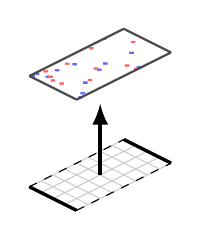
\begin{tikzpicture}[scale=0.8]
\begin{scope}[
		x=1cm,
		y=1cm,
		yshift=0,
		every node/.append style={
			yslant=0.5,xslant=-1},
		yslant=0.5,
		xslant=-1
	]
	\def\dx{0.0};
	% opacity to prevent graphical interference
	\draw[step=1.5/8, black!20!white, thin] (0,0-\dx) grid (6/4,6/8+\dx);
	%defining grids
	%\draw[step=1.5, black] (0,0) grid (6,6);
	\draw[xstep=1.5, ystep=0, black, very thick] (0,0-\dx) grid
		(6/4,6/8+\dx);
	\draw[dashed, xstep=6, ystep=1.5/2, black] (0,0) grid (6/4,6/8);

	\coordinate (b) at (1.5/2, 0.75/2);

\end{scope}
\begin{scope}[
		x=1cm,
		y=1cm,
		yshift=50,
		every node/.append style={
			yslant=0.5,xslant=-1},
		yslant=0.5,
		xslant=-1
	]
	\coordinate (c) at (1.5/2, 0.75/2);

	%\fill[fill=white,fill opacity=1.0] (0,0) rectangle (6,6);
	\begin{axis}[width=3cm,height=2.35cm,
						axis lines=none,
						%hide axis,
						xmin=-1, xmax=1,
						ymin=-1, ymax=1,
						inner frame sep=0,
				]
	\addplot [blue!60!white, only marks,
		mark=*, samples=12, mark size=0.75] (rand, rand);
	\addplot [red!60!white, only marks,
		mark=*, samples=12, mark size=0.75] (rand, rand);
	\end{axis}
	%\draw[step=1.5, black, thick] (0,0) grid (6,6);
	\draw[xstep=1.5, ystep=1.5/2, black!70!white, thick] (0,0) grid (6/4,6/8);
	%\draw[dashed,xstep=6, ystep=1.5, black, thick] (0,0) grid (6,6);


	\coordinate (O) at (1.5+0.5, 0.75+0.5);
\end{scope}

%\draw[-latex,very thick] (c)+(1,2) node[above]{Plasma chunk}
%				to[out=-90,in=90] (c);
%\draw[-latex,very thick,shorten >=3pt] (b)+(-1.5,-1) node[below]{Block}
%				to[out=90,in=180+45] (b);
\draw[-latex,ultra thick,shorten >=0.5cm]
	(b) to[out=90,in=-90] (c);
%	(b) to[out=90,in=-90]  node[midway,right]{Interpolation} (c);

\begin{scope}[
		y={(-1cm,0.5cm)},x={(1cm,0.5cm)}, z={(0cm,1cm)},
	]
%	\coordinate (O) at (-3, 3.5, 0);
%	\draw[-latex] (O) -- +(1, 0,  0) node [right] {$x$};
%	\draw[-latex] (O) -- +(0, -1, 0) node [right] {$y$};
%	\coordinate (O) at (-0.75, -0.75, 0);
%	\draw[-latex] (O) -- +(-1, 0,  0) node [left] {$y$};
%	\draw[-latex] (O) -- +(0, -1, 0) node [right] {$x$};
\end{scope}
\end{tikzpicture}
%\caption{Interpolation of the electric field $\E$ to the particles in a chunk.}
%\label{fig:interpolation-E}
\end{wrapfigure}
%\end{figure}%}}}
%
Once the electric field of a chunk is ready, the value is interpolated at the 
particle locations. The force will be obtained in the next step from the 
interpolated electric field in each particle.

Each chunk can be processed independently by one task, but a \texttt{inout} 
dependency must be added to ensure the order of execution of a chunk is done 
after the electric field is computed, as observed in the 
listing~\ref{lst:interpolate-E}.
%
\begin{figure}[ht]%{{{
\begin{lstlisting}[
label={lst:interpolate-E},
caption={Interpolation of the electric field $\E$ at particle position.}]
for(i=0; i<sim->plasma.nchunks; i++)
{
	chunk = &sim->plasma.chunks[i];
	#pragma oss task inout(*chunk) label(chunk_E)
	{
		for(is=0; is<chunk->nspecies; is++)
		{
			particle_set_E(sim, chunk, is);
		}
	}
}
\end{lstlisting}
\end{figure}%}}}
%
\subsection{Particle mover}

The force acting on each particle is obtained as described in the 
equation~\ref{eq:force}, as the combination of the electric and magnetic forces.  
The electric term is computed from the interpolated electric field at the 
particle locations and each chunk can begin the process as soon as the 
interpolation process has finished.

A task is created for each chunk, and the particles are moved accordingly to the 
obtained force. The Boris integrator described in the section~\ref{sec:boris} is 
used to accurately position the particles. An \texttt{inout} dependency is added 
to each chunk to guarantee the order of execution: after the electric field is 
interpolated in the particles, as shown in the listing~\ref{lst:particle-mover}.
%
\begin{figure}[ht]%{{{
\begin{lstlisting}[
label={lst:particle-mover},
caption={Movement of particles based on the interpolated field $\E$.}]
for(i=0; i<sim->plasma.nchunks; i++)
{
	chunk = &sim->plasma.chunks[i];
	#pragma oss task inout(*chunk) label(chunk_x_update)
	{
		for(is=0; is<chunk->nspecies; is++)
		{
			particle_x_update(sim, chunk, is);
		}
	}
}
\end{lstlisting}
\end{figure}%}}}

%\setcounter{chapter}{9}
\chapter{Communication}
\label{ch:comm}

Different communications are detailed in this chapter, such as particle and 
frontier communications.

\section{Particle communication}

When the particles are moved, due to the interaction with the electric field and 
the magnetic field, their position can exceed the boundaries of the chunk where 
they reside. After updating the position of each particle, the ones that exceed 
the chunk must be translated to the correct one. The time step is lowered to 
ensure that a particle can only travel at most one chunk per iteration, so we 
only need local communications, which are done in two stages: first the 
particles are moved in the X dimension, then in the Y. Several steps are 
required in each stage.

\subsection{Exchange in X}
\label{sec:exchange-x}

%TODO Place figure to describe the movement
All chunks in the X dimension reside in one MPI process, so the exchange of 
particles can be done by shared memory. Care must be taken to avoid concurrent 
writes in the same chunk by different tasks. The proposed solution avoids the 
problem by using temporal queues in each chunk. The process can be described in 
the following steps:
%
\begin{enumerate}
\item \texttt{collect\_particles\_x}: Out of bound particles in the X direction 
are extracted from the chunk and placed in the correct target chunk queue for 
local exchange.
\item \texttt{exchange\_particles\_x}: Each chunk looks for particles in the 
neighbour chunks target queues and moves them to itself.
\end{enumerate}
%
Usually only two target queues are required for each chunk, as the particles can 
only move one chunk per iteration. However, in the initial iteration after the 
initialization of the particle positions, they can move to any other chunk, and 
the process is subsequently more computationally expensive. We will only focus 
in the general case involving only the two neighbours, as the initialization 
iteration can be disregarded when comparing the time against the whole 
simulation.

The execution order and mutual exclusion of these two phases should be 
guaranteed by means of a synchronization mechanism. Each step can be implemented 
using OmpSs-2 tasks with dependencies, in order to exploit local parallelism.  
One task collects the particles out of the chunk in the corresponding queues, so 
it needs to access only the current chunk.
%
\begin{lstlisting}[caption={Collect particles in the X direction.}]%{{{
for(i = 0; i < plasma->nchunks; i++)
{
	chunk = &plasma->chunks[i];
	/* Place each particle outside a chunk in the X dimension, in
	 * the lout list */
	#pragma oss task inout(*chunk) label(collect_particles_x)
	for(is = 0; is < sim->nspecies; is++)
	{
		collect_particles_x(sim, chunk, is, global_exchange);
	}
}
\end{lstlisting}%}}}
%
The execution of the corresponding exchange particle tasks will start only if 
the collecting step has finished in the neighbour chunks, as otherwise the 
queues are still being written. These dependencies must be placed in all the 
involved chunks.
%
\begin{lstlisting}[caption={Exchange of particles in X}]%{{{
for (i = 0; i < plasma->nchunks; i++)
{
	chunk = &plasma->chunks[i];
	...

	#pragma oss task inout(*chunk) \
@          inout(*prev_chunk) inout(*next_chunk) \
@          label(exchange_particles_x)
	{
		/* Only the two neighbours are needed */
		concat_particles(chunk, prev_chunk);
		concat_particles(chunk, next_chunk);
	}
}
\end{lstlisting}%}}}
%
Notice that in the first iteration the exchange step must wait for all the 
collecting tasks to finish, as the particles can be moved to any chunk, and thus 
we expect to see a slower iteration than the rest of the simulation. In the 
following steps, only the next and previous chunk are required to finish the 
exchange process.

\begin{figure}[h]%{{{
	\centering
	\subfloat[Chain of dependencies observed]{
		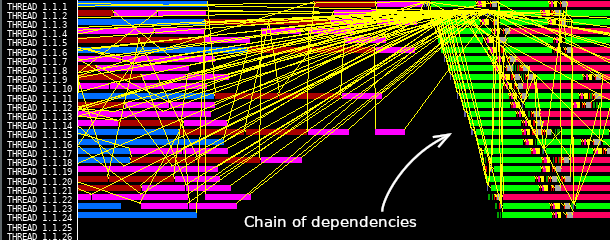
\includegraphics[width=0.7\textwidth]{chain}
		\label{fig:chain}
	}
	\\
	\subfloat[The chain has been corrected]{
		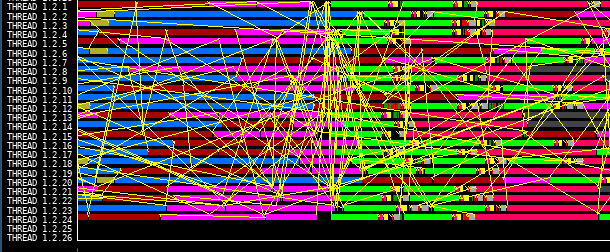
\includegraphics[width=0.7\textwidth]{no-chain}
		\label{fig:no-chain}
	}
	\caption{Comparison of two \texttt{paraver} traces using coloring tasks for 
	communication.}
\end{figure}%}}}
%
However, there is a problem with the previous loop: as we create the 
dependencies with the next chunk before the next task is created, we are 
building a chain of dependencies which leads to a sequential execution.  Using 
\texttt{paraver} we can clearly see the chain in the trace graph, shown in the 
figure~\ref{fig:chain}, where no task can run in parallel until the previous one 
finishes.  One solution to alleviate this problem is the use of a coloring 
technique, where each task is assigned a color.  Then all tasks of the same 
color are created first, then the ones with the next color and so on.
%
\begin{figure}[ht]%{{{
\centering
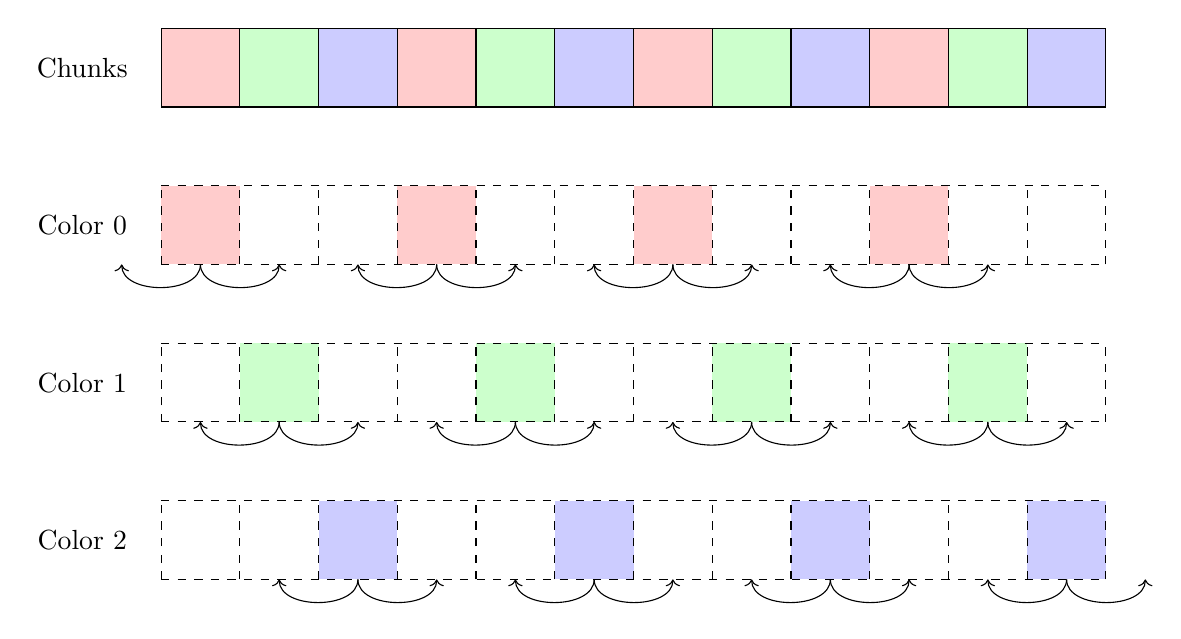
\begin{tikzpicture}
\node at (-1,2.5) {Chunks};
\foreach \x in {0,3,...,9} {
	\fill[red!20](\x,2) rectangle +(1,1);
	\fill[green!20](\x+1,2) rectangle +(1,1);
	\fill[blue!20](\x+2,2) rectangle +(1,1);
}
\draw[step=1] (0,2) grid +(12,1);

\foreach \y\mycol [evaluate=\y as \yy using int(\y/2)]
	in {0/red,2/green,4/blue} {
	\node at (-1,-\y+0.5) {Color \yy};
	\foreach \x in {0,3,...,9} {
		\fill[\mycol!20](\x+\yy,-\y) rectangle +(1,1);
	}
	\foreach \x in {0,3,...,9} {
		\draw[->] (\x,-\y)++(\yy,0)++(.5,0) to[out=-90,in=-90] +(1,0);
		\draw[->] (\x,-\y)++(\yy,0)++(.5,0) to[out=-90,in=-90] +(-1,0);
	}
	\draw[step=1,dashed] (0,-\y) grid +(12,1);
}
%\draw[dashed,step=0.5] (0,0) grid (8,-0.5);
%\draw[thick](0,0) rectangle (8,4);
%
%\fill[white, radius=0.8](4,2) circle;
%\node (center) at (4,2) {\huge $E_y$};
%
%\coordinate (ghost) at (-0.1, -0.25);
%\node (g0r) [left of=ghost, xshift=-0.2cm] {Ghost};
%\draw[->] (g0r) -- (ghost0);
%
%\coordinate (gghost) at (8.1, -0.25);
%\node (ggr) [white,right of=gghost, xshift=0.2cm] {Ghost};
%\draw[white,->] (ggr) -- (gghost);
\end{tikzpicture}
\caption{The coloring technique shown with 12 chunks where the 12 tasks are 
created with 3 colors.}
\label{fig:coloring}
\end{figure}%}}}
%
With three colors we ensure that the two tasks of the same color can run in 
parallel without concurrent access to the same chunk, as can be seen in the 
figure~\ref{fig:coloring}.
%
\begin{lstlisting}[caption={Exchange of particles in X using the coloring %{{{
technique}]
max_color = 3;

for(color = 0; color < max_color; color++)
{
	/* Use coloring to prevent a chain of dependencies */
	for(i = color; i < plasma->nchunks; i+=max_color)
	{
		chunk = &plasma->chunks[i];
		...

		#pragma oss task inout(*chunk) \
	@              inout(*prev_chunk) inout(*next_chunk) \
	@              label(collect_local_particles)
		{
			/* Only the two neighbours are needed */
			concat_particles(chunk, prev_chunk);
			concat_particles(chunk, next_chunk);
		}
	}
}
\end{lstlisting}%}}}
%
In the figure~\ref{fig:no-chain} it can be observed how the chain has now 
disappeared, and the gaps are now fully covered by tasks running in parallel.

This technique can be expressed without extra work, by using the directive 
\texttt{commutative}, which acts similarly as \texttt{inout} but can be executed 
in any order. Then, once a task begins execution, locking the next chunk, other 
unordered chunk can be executed in any order, if their neighbour chunks are 
unlocked.
%
\begin{lstlisting}[caption={Exchange of particles in X using the %{{{
\texttt{commutative} directive.}]
for(i = 0; i < plasma->nchunks; i++)
{
	chunk = &plasma->chunks[i];
	...

	#pragma oss task commutative(*chunk, *prev_chunk, *next_chunk) \
@              label(collect_local_particles)
	{
		/* Only the two neighbours are needed */
		concat_particles(chunk, prev_chunk);
		concat_particles(chunk, next_chunk);
	}
}
\end{lstlisting}%}}}
%
Once all exchange tasks are completed, all particles are now placed in the 
correct chunk in the X dimension, and only the Y movement is left.

\subsection{Exchange in Y}
%TODO Place figure to describe the movement
Once the particles are placed in the correct chunk in the X dimension, the 
displacement to the correct chunk in the Y dimension involves sending the 
particles to another MPI process. The steps can be resumed as:
%
\begin{enumerate}
\item \texttt{collect\_particles\_y}: Place each particle out of the chunk 
bounds in a queue (one for each target destination).
\item \texttt{pack\_particles\_y}: Pack the particles to be sent to the 
neighbour chunk in a message.
\item \texttt{send\_particles\_y}: Send the packed particles to each neighbour.
\item \texttt{recv\_particles\_y}: Receive the message with the packed 
particles.
\item \texttt{unpack\_particles\_y}: Unpack the particle message and place the 
particles in the chunk.
\end{enumerate}
%
\begin{figure}
\centering
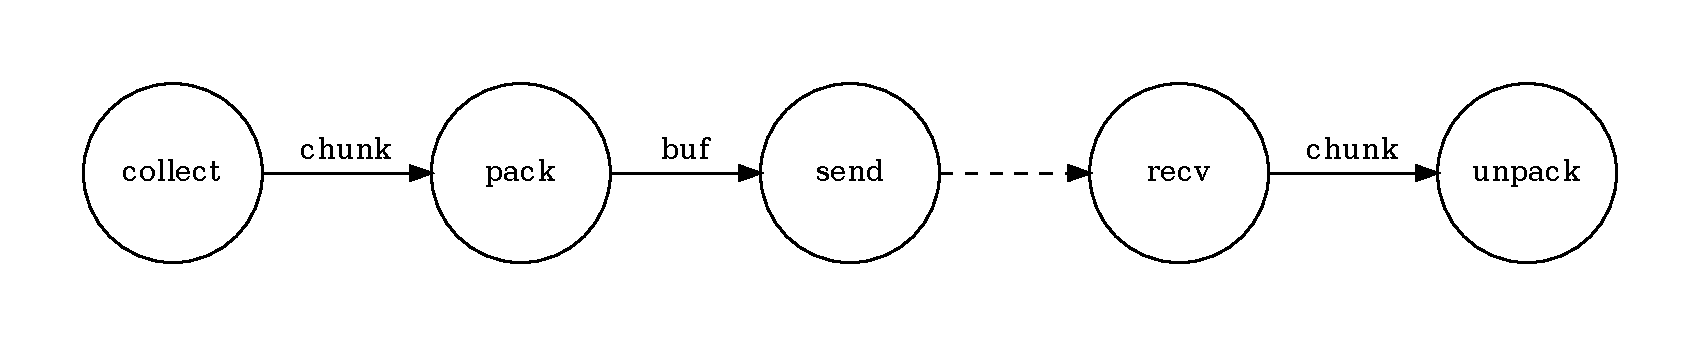
\includegraphics[width=\textwidth]{comm-particles.pdf}
\caption{Graph of task and dependencies of particle communication in Y: Solid 
arrows indicate a data dependency, dashed arrows show a creation dependency 
order.}
\label{fig:comm_y}
\end{figure}
%
Similarly as for the horizontal direction, the particles exceeding the limits of 
each chunk in the Y dimension are placed in a queue.  Once the particles are 
identified within a chunk, they are packed in a message in a contiguous memory 
region. This buffer is then sent using \texttt{MPI\_Send} to the neighbour 
process.

The reception process works in the opposite order: each chunk receives the 
communication of the neighbour chunks in the vertical direction. Once a message 
is received is unpacked and the particles are added to the chunk. In the 
diagram~\ref{fig:comm_y} the dependencies of each step are shown in a graph.

Notice that all the MPI communication is independent of the neighbour chunks in 
the horizontal direction, and can be fully parallelized. Some constraints must 
be added to coordinate the vertical communications to guarantee that no 
simultaneous writes occur in the same chunk.

\begin{lstlisting}[caption={Communication of particles in the Y direction.}]
for(i = 0; i < plasma->nchunks; i++)
{
	chunk = &plasma->chunks[i];

	/* Collect particles in a queue that need to change chunk */
	#pragma oss task inout(*chunk) label(collect_particles_y)
	for(is = 0; is < sim->nspecies; is++)
	{
		collect_particles_y(sim, chunk, is, global_exchange);
	}

	/* Prepare the packet to be sent to the neighbour */
	#pragma oss task inout(*chunk) label(pack_particles_y)
	pack_particles_y(sim, chunk, i, global_exchange);

	/* Finally send the packet */
	#pragma oss task in(*chunk) label(send_particles_y)
	send_particles_y(sim, chunk, i, global_exchange);

	/* The tasks are created inside depending on
	 * whether we use MPI or TAMPI */
	recv_particles_y(sim, chunk, global_exchange);
}
\end{lstlisting}

\subsection{Mitigation of deadlocks with TAMPI}

When using MPI to exchange particles between processes, the design must be done 
with special care to avoid deadlocks: Assume each chunk tags the message with 
the chunk index, so the receiver can filter messages which are not from the 
vertical direction. Also, consider that we have multiple chunks, more than the 
number of CPUs available, so there are some task that cannot run in parallel and 
must wait.

It may happen that some task already sent messages and has reached the reception 
stage: it is waiting to continue and subsequently blocking the task until a 
message with the correct tag arrives. But other tasks may be waiting for the CPU 
to begin the communication and didn't send yet any message. When no CPUs are 
left, a deadlock is produced as represented in the 
figure~\ref{fig:comm_deadlock}, where each chunk is represented by a box node 
and the edges show which messages were sent.
%
\begin{figure}
\centering
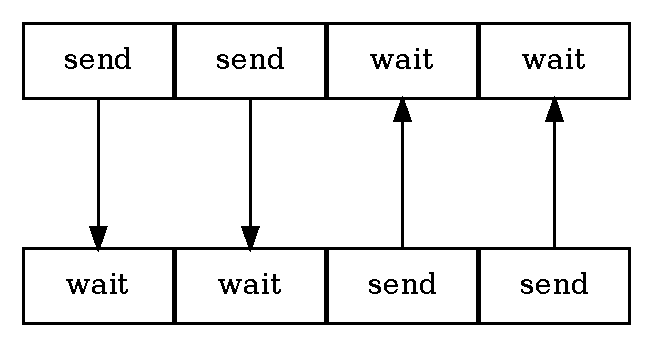
\includegraphics[width=0.4\textwidth]{deadlock-particles.pdf}
\caption{Deadlock at particle exchange in Y, where each message has a different 
tag.}
\label{fig:comm_deadlock}
\end{figure}

In order to palliate the deadlock, we can avoid using the tag as a filter, so 
once the sending is complete, the task waits for the reception of particles from 
any other chunk.  With this method, it is guarantee that no deadlock can occur, 
as before a task enters the waiting state, after sending the message, another 
task will be unlocked and can resume the execution:
%
\begin{lstlisting}[caption={Reception of particles with MPI}]
#pragma oss task inout(*chunk) weakinout(chunk[0:Nc-1]) \
@    commutative(*sim) label(recv_particle_packet_MPI)
{
	comm_packet_t *pkt;
	...

	MPI_Probe(MPI_ANY_SOURCE, tag, MPI_COMM_WORLD, &status);

	source = status.MPI_SOURCE;
	MPI_Get_count(&status, MPI_BYTE, &size);

	pkt = safe_malloc(size);

	MPI_Recv(pkt, size, MPI_BYTE, source, tag, MPI_COMM_WORLD,
			MPI_STATUS_IGNORE);

	recv_chunk = &sim->plasma.chunks[pkt->dst_chunk[X]];

	#pragma oss task inout(*pkt) inout(*recv_chunk) label(unpack_comm_packet)
	{
		unpack_comm_packet(sim, recv_chunk, pkt);
		free(pkt);
	}
}
\end{lstlisting}
%
It must be enforced that the calls to \texttt{MPI\_Recv} and \texttt{MPI\_Probe} 
are done in mutual exclusion, as otherwise another task could receive the 
message between the tho calls. The dependency with the sentinel \texttt{*sim} 
avoids the problem, which is released as soon as the packet is received. Notice 
that, in order to create a nested task to process the chunk stated in the 
packet, we must indicate in the \texttt{weakinout} directive all posible chunks 
that may be selected. Then, only one will be used by the child task to unpack 
the particles.

The downside of the described mechanism is the implicit complexity and the 
amount of extra work needed to ensure a deadlock free execution, which can be 
avoided with TAMPI. The deadlock is mitigated not by removing the tag, which 
filters the chunk, but by setting the task to sleep once it enters in the 
waiting state, so other tasks can begin the execution. The TAMPI library 
intercepts the calls to MPI and informs the OmpSs-2 scheduler that the task can 
be put to sleep.

Using TAMPI only requires a minor modifications with respect to the original 
implementation: the message size must be known at the receiver. The current 
version of TAMPI doesn't include \texttt{MPI\_Probe} in the family of 
intercepted functions. The MPI version first probes for the message to get the 
length and then allocates a buffer to hold the entire message. A buffer of known 
size may be used to hold the parts of the message while is being send. The 
message includes the complete size of the message in the header, so after the 
reception of the first message, the whole buffer can be allocated.

\begin{lstlisting}[caption={Reception of particles with TAMPI}]
#pragma oss task out(*pkt) inout(*chunk) label(recv_particle_packet_TAMPI)
{
	...

	size = BUFSIZE;
	pkt = safe_malloc(size);
	MPI_Recv(pkt, size, MPI_BYTE, proc, tag, MPI_COMM_WORLD,
			MPI_STATUS_IGNORE);

	/* If more data is comming, realloc and receive it */
	if(pkt->size > size)
	{
		done = size;
		size = pkt->size;
		parts_left = (size - done + (BUFSIZE - 1)) / BUFSIZE;

		/* If the packet is only a fragment, continue until we
		 * fill the whole buffer */
		pkt = realloc(pkt, size);
		if(!pkt) abort();

		requests = safe_malloc(parts_left * sizeof(MPI_Request));

		/* Recv by chunks */
		for(j=0,ptr=pkt,i=BUFSIZE; i<size; j++, i+=BUFSIZE)
		{
			left = size - i;
			if(left > BUFSIZE)
				left = size;

			MPI_Irecv(ptr+i, left, MPI_BYTE, proc, tag,
					MPI_COMM_WORLD, &requests[j]);
		}

		MPI_Waitall(parts_left, requests, MPI_STATUSES_IGNORE);
		free(requests);
	}
	unpack_comm_packet(sim, chunk, pkt);
	free(pkt);
}
\end{lstlisting}

Note that all communications are done with \texttt{MPI\_BYTE}, sending the 
packed structures as an array of bytes. This methods of transmission sends the 
data ``as-is''---MPI doesn't perform any endianness adjustment. We assume the 
simulation will run within nodes with the same endianness, otherwise MPI will 
need information of each field or a manual process must be added before the 
message is unpacked. Additionally, the structures sent over MPI are packed to 
avoid any holes in the buffer sent.

\section{Field communication}

Each MPI process holds a block with the different fields of the assigned region 
of space. Due to the interpolation process some elements of the neighbour fields 
are needed to complete the interpolation, which implies that additional 
communication is needed.

\subsection{Charge density $\rho$}

Following the order of the simulation, first the $\rho$ field is updated, where 
all particles deposit the charge. Given a $\rho$ field of size $(n_x, n_y)$ an 
extra row $\rho_{n_y}$ is added to hold the first row of $\rho$ of the next 
block $\rho_0$, as shown in the figure~\ref{fig:field_rho}. Notice that an extra 
padding is required by the FFTW library, to accommodate intermediate results, 
and must be taken into account when designing the communications.
%
\begin{figure}[ht]
\centering
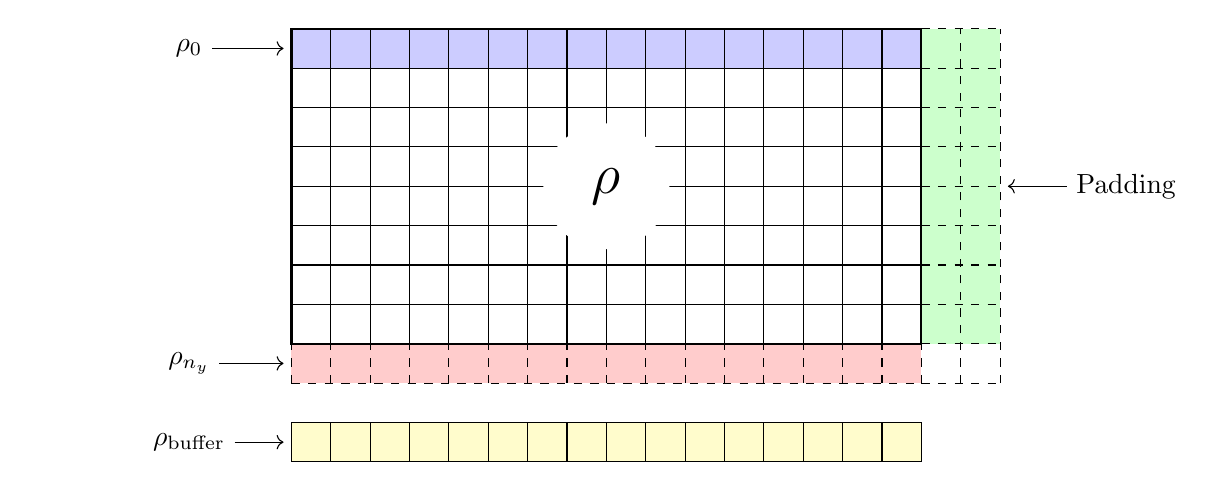
\begin{tikzpicture}
\fill[blue!20](0,3.5) rectangle (8,4);
\draw[step=0.5] (0,0) grid (8,4);
\fill[red!20](0,0) rectangle (8,-0.5);
\draw[dashed,step=0.5] (0,0) grid (8,-0.5);
\fill[green!20](8,0) rectangle (9,4);
\draw[dashed,step=0.5] (8,-0.5) grid (9,4);
\draw[thick](0,0) rectangle (8,4);

\coordinate (first) at (-0.1, 3.75);
\fill[white, radius=0.8](4,2) circle;
\node (center) at (4,2) {\huge $\rho$};
\node (fr) [left of=first, xshift=-0.2cm] {$\rho_0$};
\draw[->] (fr) -- (first);

\coordinate (ghost) at (-0.1, -0.25);
\node (gr) [left of=ghost, xshift=-0.2cm] {$\rho_{n_y}$};
\draw[->] (gr) -- (ghost);

\coordinate (fft) at (9.1, 2);
\node (fft-label) [right of=fft, xshift=0.5cm] {Padding};
\draw[->] (fft-label) -- (fft);

\coordinate (gfft) at (-1.1, 2);
\node (gfft-label) [white,left of=gfft, xshift=-0.5cm] {Padding};
\draw[white,->] (gfft-label) -- (gfft);

\fill[yellow!20](0,-1) rectangle (8,-1.5);
\draw[step=0.5] (0,-1) grid (8,-1.5);
\coordinate (buf) at (-0.1, -1.25);
\node (br) [left of=buf, xshift=-0.2cm] {$\rho_\text{buffer}$};
\draw[->] (br) -- (buf);
\end{tikzpicture}
\caption{The field $\rho$ with the padding}
\label{fig:field_rho}
\end{figure}

Each process sends $\rho_{n_y}$ to the next process, and receives $\rho_0$ from 
the previous one. The size of the message is constant and known beforehand, so 
it can the be stored in the same buffer $\rho_\text{buffer}$ in each iteration, 
which is added to $\rho_0$ to finally complete $\rho$ where the ghost is no 
longer needed.

If the ghost is sent before we begin the reception process, we can reuse 
$\rho_{n_y}$ to hold also $\rho_\text{buffer}$. But the communications use 
non-blocking communications, which may not finish when the process reaches the 
reception step, so an additional buffer is used instead---a technique known as 
double buffering.  Before each send the status of the previous request is 
tested, and in case is not yet finished, we wait before continue. The two main 
functions \texttt{comm\_mat\_send} and \texttt{comm\_mat\_recv} are used to 
transfer a buffer of floating point numbers.

\begin{lstlisting}
int comm_mat_send(sim_t *sim, double *data, int size, int dst,
	int op, int dir, MPI_Request *req)
{
	int tag = compute_tag(op, sim->iter, dir, COMM_TAG_DIR_SIZE);

	if(*req)
		MPI_Wait(req, MPI_STATUS_IGNORE);

	return MPI_Isend(data, size, MPI_DOUBLE, dst, tag,
		MPI_COMM_WORLD, req);
}

int comm_mat_recv(sim_t *sim, double *data, int size, int dst,
	int op, int dir)
{
	int tag = compute_tag(op, sim->iter, dir, COMM_TAG_DIR_SIZE);

	return MPI_Recv(data, size, MPI_DOUBLE, dst, tag,
		MPI_COMM_WORLD, MPI_STATUS_IGNORE);
}
\end{lstlisting}

\subsection{Electric potential $\phi$}

After the solver, the result is stored in a similar way as $\rho$, with padding 
at the right. However, now we have more ghosts at the top and at the bottom of 
$\phi$, as they will be needed to compute the electric field $\E$. In the 
figure~\ref{fig:field_phi} the different regions can be seen: In blue the ones 
which will be send, $\phi_{0}$ and $\phi_{1}$ to the previous process to fill 
$\varphi_{n_y}$ and $\varphi_{n_y + 1}$, and $\phi_{n_y - 1}$ to be sent to the 
next process, to fill $\varphi_{-1}$.
%
\begin{figure}[ht]
\centering
\begin{tikzpicture}
\fill[red!20](0,4) rectangle (8,4.5);
\draw[dashed,step=0.5] (0,4) grid (8,4.5);
\fill[blue!20](0,3) rectangle (8,4);
\fill[blue!20](0,0) rectangle (8,0.5);
\draw[step=0.5] (0,0) grid (8,4);
\fill[red!20](0,0) rectangle (8,-1);
\draw[dashed,step=0.5] (0,0) grid (8,-1);
\fill[green!20](8,0) rectangle (9,4);
\draw[dashed,step=0.5] (8,-1) grid (9,4.5);
\draw[thick](0,0) rectangle (8,4);

\fill[white, radius=0.8](4,2) circle;
\node (center) at (4,2) {\huge $\phi$};

\coordinate (first) at (-0.1, 3.75);
\node (fr) [left of=first, xshift=-0.2cm] {$\phi_0$};
\draw[->] (fr) -- (first);

\coordinate (second) at (-0.1, 3.25);
\node (sr) [left of=second, xshift=-0.2cm] {$\phi_1$};
\draw[->] (sr) -- (second);

\coordinate (last) at (-0.1, 0.25);
\node (sr) [left of=last, xshift=-0.2cm] {$\phi_{n_y - 1}$};
\draw[->] (sr) -- (last);

\coordinate (ghost-1) at (-0.1, 4.25);
\node (g-1r) [left of=ghost-1, xshift=-0.2cm] {$\varphi_{-1}$};
\draw[->] (g-1r) -- (ghost-1);
\coordinate (ghost0) at (-0.1, -0.25);
\node (g0r) [left of=ghost, xshift=-0.2cm] {$\varphi_{n_y}$};
\draw[->] (g0r) -- (ghost0);
\coordinate (ghost1) at (-0.1, -0.75);
\node (g1r) [left of=ghost1, xshift=-0.2cm] {$\varphi_{n_y + 1}$};
\draw[->] (g1r) -- (ghost1);

\coordinate (fft) at (9.1, 2);
\node (fft-label) [right of=fft, xshift=0.5cm] {Padding};
\draw[->] (fft-label) -- (fft);

\coordinate (gfft) at (-1.1, 2);
\node (gfft-label) [white,left of=gfft, xshift=-0.5cm] {Padding};
\draw[white,->] (gfft-label) -- (gfft);

\end{tikzpicture}
\caption{The electric potential $\phi$ with the ghost rows (red) and padding 
(green)}
\label{fig:field_phi}
\end{figure}
%
Notice the use of the notation $\varphi$ to denote the ghosts and $\phi$ the 
rows of the actual field.

It can be observed that the first two rows $\phi_0$ and $\phi_1$ are not 
consecutive in memory, as they have the padding at the right. To avoid two 
messages or additional copies, the two rows are sent with the padding included, 
which will be placed ``as-is'' in the receiving process at $\varphi_{n_y}$ and 
$\varphi_{n_y + 1}$, as the padding region is ignored.

\subsection{Electric field $\boldsymbol{E}$}

The electric field $\E$ can be computed from the ghosts of the electric 
potential $\phi$ without the need of extra communications. The electric field 
$E_x$ with a periodic boundary is obtained from $\phi$, as the whole space 
domain is available in the block in the $X$ dimension.
%
\begin{figure}[ht]
\centering
\begin{tikzpicture}
\draw[step=0.5] (0,0) grid (8,4);
\fill[red!20](0,0) rectangle (8,-0.5);
\draw[dashed,step=0.5] (0,0) grid (8,-0.5);

\fill[white, radius=0.8](4,2) circle;
\node (center) at (4,2) {\huge $E_y$};

\coordinate (ghost) at (-0.1, -0.25);
\node (g0r) [left of=ghost, xshift=-0.2cm] {$\mathcal{E}_y(n_y)$};
\draw[->] (g0r) -- (ghost0);

\coordinate (gghost) at (8.1, -0.25);
\node (ggr) [white,right of=gghost, xshift=0.2cm] {Ghost};
\draw[white,->] (ggr) -- (gghost);
\draw[thick](0,0) rectangle (8,4);

\end{tikzpicture}
\caption{The electric field $E_y$ with the ghost row at $n_y$ (red)}
\label{fig:field_Ey}
\end{figure}
%
In the case of $E_y$ we will need the ghost row at $n_y$, which is marked in red 
in the figure~\ref{fig:field_Ey}, in order to interpolate the electric field in 
the particles of the block. But the computation of the whole field can be 
produced from the extra ghost rows stored in $\phi$, which were precisely placed 
to avoid another communication step.

%\chapter{Analysis}


%\section{Analyze time distribution}

In order to reduce the amount of CPU time involved in each step of the 
simulation, the best strategy is to reduce the time spent in the most time 
consuming part.

The CPU time involved in each part of the simulation may depend on various 
factors, such as the number of grid points, the number of particles or the 
boundary conditions. As an example, consider a simulation with a large number of 
grid points, with few particles---the computation of the electric field 
(\texttt{field\_E}) will dominate the simulation time, as shown in the figure 
\ref{fig:cm-big-grid}. In a case of a large number of particles and a smaller 
grid, the particle interpolation (\texttt{particle\_E}) dominates the whole 
execution as seen in the figure \ref{fig:cm-lots-particles}.
%
\begin{figure}[h]
	\centering
	\subfloat[1024 particles, 512x512 grid points]{
		\includegraphics[width=0.95\linewidth]{callmap-grid512x512-n1024.png}
		\label{fig:cm-big-grid}
	}
	\\
	\subfloat[10240 particles, 64x64 grid points]{
		\includegraphics[width=0.95\linewidth]{callmap-grid64x64-n10240.png}
		\label{fig:cm-lots-particles}
	}
	\caption{Comparison of the time spent in each function at two different 
	simulations.}
\end{figure}
%
In order to optimize the general use case, different inputs will be tested and 
the main simulation steps will be characterized. Furthermore, different 
algorithms or methods may be used to improve the speed. As an example, the LU 
algorithm is compared with the spectral method MFT.

\section{Analysis with varying inputs}

\chapter{Analysis of performance}

The execution time is measured and analyzed in detail.

\section{Variables of interest}

A simple test to determine the performance of the simulator is to measure the
time per iteration (using the wall clock). The time spent in the different
stages of the simulation can also be of interest.

Consider the sequence of time per iteration (also referred simply as the time)
$T_0,\ldots,T_n$ as independent random variables from a common distribution with
an unknown mean $\mu$ and finite standard deviation $\sigma$. The sample mean
$\overline T$ can be approximated with a certain degree of confidence by a
process of sampling.

Different parameters of the simulation may affect the time mean $\mu$ and is the
objective of this chapter to find out what the relation is. The time is at least
in $O(N_p)$, as we need to iterate over each particle $N_p$. We also know that
the worst-case complexity of the FFT is in $O(N_g \log N_g)$ for $N_g$ total grid
points.

The simulator runs for at least 30 iterations, and then the standard error of 
the mean (SEM) is computed. Then in each iteration is determined if the SEM is 
below a threshold to stop the simulation. The threshold is determined so that 
when the simulation stops, the mean is has an error of at most 0.2\% with 
probability 95\%.

\subsection{Number of particles}

The number of particles $N_p$ is one of the main parameters that affect the
running time of each iteration. In order to characterize the scalability of the
application, several tests are designed with increasing number of particles, and
different metrics are compared.

The wall clock is used in the process with rank zero to measure how long takes
each iteration.

\begin{figure}[h]
	\centering
	\subfloat[Increasing number of particles]{
		\begin{tikzpicture}
		\begin{axis}[
			width=0.5\textwidth,
			xlabel=Particles $N_p$,
			ylabel=Time per iteration (s),
			grid=major]
		\addplot [only marks,error bars/y dir=both, error bars/y explicit] table [
			x index = {0},
			y index = {3},
			y error index={4},
			col sep=space] {csv/particles.csv};
		\end{axis}
		\end{tikzpicture}
	}
	\subfloat[Increasing number of grid points]{
		\begin{tikzpicture}
		\begin{axis} [
			no markers,
			grid=major,
			xlabel=Grid points $N_g$,
			ylabel=Time per iteration (s),
			width=0.5\textwidth]
		\addplot [only marks,error bars/y dir=both, error bars/y explicit] table [
			x index = {0},
			y index = {3},
			y error index={4},
			col sep=space] {csv/solver.csv};
		\end{axis}
		\end{tikzpicture}
	}
	\caption{The effect of the variables $N_p$ and $N_g$ to the time per 
	iteration. Using one process and 32 CPUs (MPI communications are not needed).}
\end{figure}

\subsection{Constant number of CPUs}

The simulator is designed to scale with the number of particles when the number 
of CPUs or process are incremented, as each chunk can be computed in parallel.  
But when the number of grid points is incremented, the FFT solver must scale 
both in the number of CPUs and processes. The FFTW library offers two 
parallelization implementations for multithreading: Using OpenMP and POSIX 
threads (pthreads). OpenMP is not compatible with OmpSs-2 as we have one runtime 
already running so the pthread implementation was tested.
%
\begin{figure}[h]
	\centering
		\begin{tikzpicture}
		\begin{axis} [
			legend pos=north west,
			xmode=log,
			log basis x=2,
			xticklabels={0,1,2,4,8,16,32},
			grid=major,
			xlabel=Number of CPUs,
			ylabel=Time per iteration (s),
			width=10cm,
			height=6cm,
			]
		\addplot+ [only marks,error bars/y dir=both, error bars/y explicit] table [
			x index = {0},
			y index = {3},
			y error index={4},
			col sep=space] {csv/fftw-sequential.csv};
		\addlegendentry{Single thread}
		\addplot+ [only marks,error bars/y dir=both, error bars/y explicit] table [
			x index = {0},
			y index = {3},
			y error index={4},
			col sep=space] {csv/fftw-threads.csv};
		\addlegendentry{Multithread}
		\end{axis}
		\end{tikzpicture}
	\caption{The number of CPUs is increased with only one process: the solver 
	cannot scale and the time per iteration increases. Configuration used: $N_p = 
	\num{5e5}$, $N_g=8192\times8192$.}
	\label{fig:fftw-time}
\end{figure}
%
Unfortunately, the FFTW library doesn't show a good speedup, in fact worsens the 
time per iteration when adding more threads with the configurations tested. In 
the figure~\ref{fig:fftw-time} it can be shown how the time grows as the number 
of CPUs increases.
%
The FFTW documentation warns about this problem, claiming that it can only 
improve the time with large enough matrices:
%
\begin{displayquote}
A shared-memory machine is one in which all CPUs can directly access the same 
main memory, and such machines are now common due to the ubiquity of multi-core 
CPUs. FFTW’s multi-threading support allows you to utilize these additional CPUs 
transparently from a single program. However, this does not necessarily 
translate into performance gains---when multiple threads/CPUs are employed, 
there is an overhead required for synchronization that may outweigh the 
computational parallelism. Therefore, you can only benefit from threads if your 
problem is sufficiently large.
\end{displayquote}
%
However, larger matrices are not useful to get more precise results, as we 
rather prefer an increase in the number of particles than in grid points.


\begin{figure}[h]
	\centering
	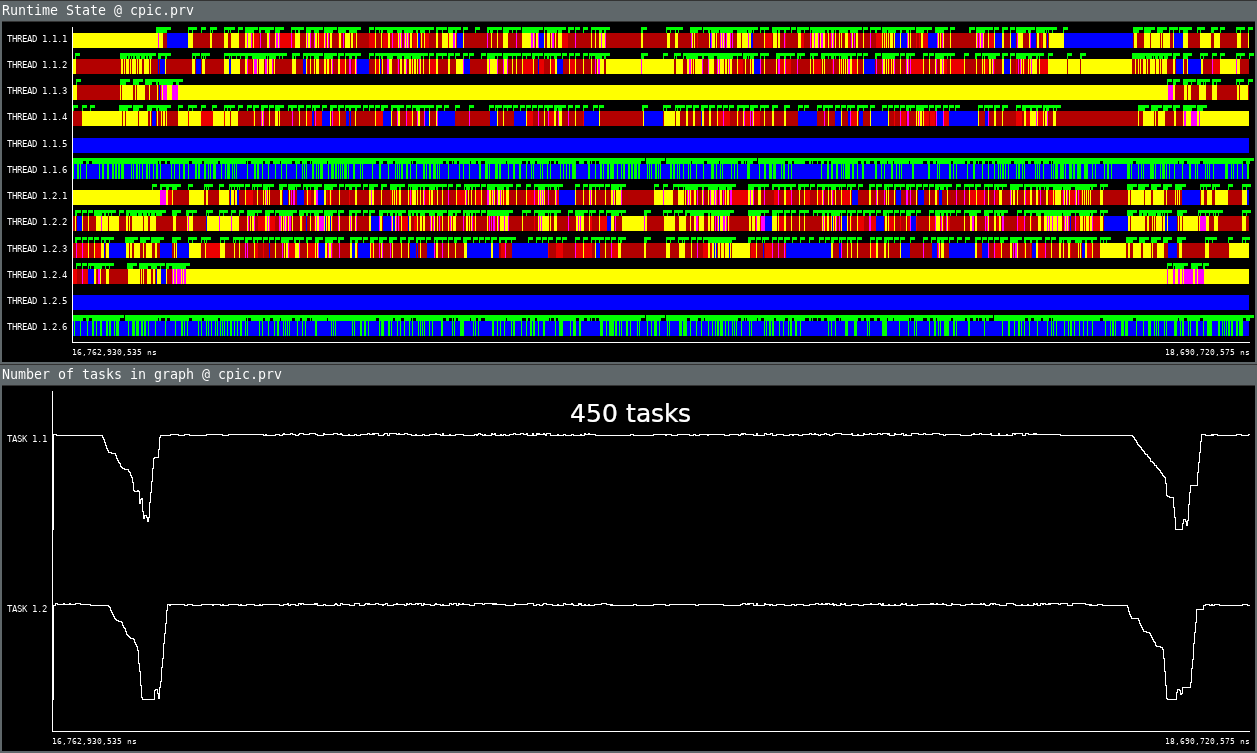
\includegraphics[width=0.95\linewidth]{fftw-ompss2.png}
	\caption{Tasks created inside the FFTW when using OmpSs-2: Up to 450 tasks are 
	created in rapid succession, with only 4 CPUs and 2 processes.}
	\label{fig:fftw-ompss2}
\end{figure}

In order to avoid a scalability problem, another approach was tested: Add 
support for OmpSs-2~in the FFTW to enable multithreading, following the same 
structure as OpenMP. The results obtained were similar as with the pthread case, 
but more insight was gained in how the task were created. It shown that the 
overhead added by the large amount of created and destructed quick tasks 
outweight any benefit that could be gained by multithreading.


We can mitigate the effect of the scaling by increasing the number of processes.  
In order to evaluate which ratio of processes and CPUs yields the best 
performance several configurations are tested. With a fixed number of maximum 
CPUs available set to 32, we increase the number of processes while we reduce 
the CPUs per process.


\begin{figure}[h]
	\centering
		\begin{tikzpicture}
		\begin{axis} [
			legend pos=outer north east,
			xmode=log,
			log basis x=2,
			xticklabels={0,1,2,4,8,16},
%			xticklabel style={
%			/pgf/number format/precision=3,
%			/pgf/number format/fixed},
			grid=major,
			xlabel=Number of CPUs per process,
			ylabel=Time per iteration (s),
			width=0.5\textwidth]
		\addplot [ybar stacked, fill=red!30!white] table [
			x index = {0},
			y index = {10},
			col sep=space] {csv/constant-cpus.csv};
		\addlegendentry{Solver}
		\addplot [ybar stacked, fill=blue!30!white] table [
			x index = {0},
			y index = {11},
			col sep=space] {csv/constant-cpus.csv};
		\addlegendentry{Particles}
		\addplot [only marks,error bars/y dir=both, error bars/y explicit] table [
			x index = {0},
			y index = {5},
			y error index={6},
			col sep=space] {csv/constant-cpus.csv};
		\addlegendentry{Total}
		\end{axis}
		\end{tikzpicture}
	\caption{The number of CPUs per process is incremented while reducing the 
	number of processes (the total number of CPUs is set to 32 and is kept 
	constant).  The time per iteration is measured, which leads to a 
	characteristic U shape.}
\end{figure}




%\chapter{Configuration}
\label{ch:config}

\chapter{Discussion}
\label{ch:discussion}


\section{Conclusions}

The presented simulator faces challenging computational patterns that are 
representative in real case scenarios, which were the main aim of this work. 

Firstly, when using dependencies in the neighbour chunks a chain of dependencies 
disallows the parallel execution and has been solved by the use of two different 
techniques: the coloring of the chunks and the \texttt{commutative} directive.

The model of communications used with MPI, consisting in the use of probe and 
receive can be proposed to the inclusion into TAMPI, as the current solution 
requires minor modifications.

The use of TAMPI leads to a more efficient execution and improved performance, 
as the runtime can fully optimize the time by doing other tasks, and avoiding 
the waiting time between MPI calls.

Using the model provided by OmpSs-2 based on tasks, the parallelization of the 
different stages of the simulation was possible. The only step which continues 
to be sequential is the solver, for which a proposed solution is described for 
the future work.

\section{Future work}

The main problem to be solved in the simulator is to address the scalability 
issues presented by the FFT, as the mitigations tested don't provide a good 
solution. One possibility is the interoperability of the OmpSs-2 runtime, 
nanos6, with external MPI processes with an additional mechanism of 
synchronization. In this way, the simulator can be fully parallelized, even at 
the core level. A step by step scheme for a configuration with $C$ CPUs 
available per node and $N$ nodes, is outlined as follows:
%
\begin{enumerate}
\item Begin the simulation as usual creating $P=N$ master processes, each with 
at least $N_c \ge 2C$ plasma chunks, to exploit the local parallelism of the $C$ 
CPUs.
\item Place the fields $\rho$, $\phi$ and $\E$ in a shared memory region, 
accessible by other child processes.
\item Create $K$ MPI child processes in each master process, with access to the 
shared memory and let them wait on a condition variable or the reception of a 
MPI message.  Ensure the number of points $N_g$ in the vertical dimension is 
divisible by $KP$.
\item Continue the simulation until it reaches the solver stage.
\item Ensure all tasks are finished, and wake all the child processes and then 
wait for them to finish.
\item In each child process execute the distributed FFTW with $KP$ processes, 
and use the shared memory to access the fields.
\item Once the FFT finishes, signal the master and put each child process to 
sleep again, waiting for a signal.
\item In the master process, the $\phi$ field is now ready in the shared memory 
region. If the simulation is not finished, go to step 4.
\end{enumerate}
%
The key concept is that we are moving temporally the threads of the OmpSs-2 
runtime away from the CPUs to let the MPI processes of the FFTW take control of 
the full parallelism using all the available CPUs. No change is needed in the 
FFTW library, and this method may benefit other programs with similar issues.

On the other hand, the physical results must be validated with a direct 
comparison with other simulators, as is very easy simulate non-realistic 
behavior without noticing. The different validation techniques provide some 
ground that the simulation follows the expected behavior, but don't guarantee 
any correctness.

Additionally, there are a large list of improvements that were planned and may 
be tested in a future work:

\begin{itemize}
\item Introduce more than 2 dimensions.
\item Fully electromagnetic simulation.
\item Relativistic particle movement.
\item Heterogeneous architecture (GPU+CPU).
\item Better energy conserving codes.
\item Test other interpolation methods (reduce noise at computational cost).
\item Replace simulation units, so we avoid factor multiplications.
\item Visualization of big simulations (paraview).
\item Introduction of probe+receive operations in TAMPI.
\end{itemize}


%
%\chapter{Results}
%
%\chapter{Conclusions}

\bibliographystyle{siam}
\bibliography{bib}

%\epigraph{So I wish to you the good luck to be somewhere where you are free to 
%maintain the kind of integrity I have described, and where you do not feel 
%forced by a need to maintain your position in the organization, or financial 
%support, or so on, to lose your integrity. May you have that freedom.}{Cargo 
%Cult Science, Caltech (1974)---\textit{Richard P. Feynman}}

\end{document}
